\documentclass[bibtotoc,parskip=full]{scrreprt}

\usepackage[utf8]{inputenc}
\usepackage[T1]{fontenc}
\usepackage[english]{babel}
\usepackage{graphicx}
\usepackage{lipsum}
\usepackage{tabularx}
\usepackage{booktabs}
\usepackage[toc,page]{appendix}

% Add dummy phantomsection for use
\providecommand\phantomsection{}

% Referemces
\usepackage[backend=biber,style=apa]{biblatex}
\addbibresource{bibliography.bib}
%\usepackage{csquotes}

% glossaries
\usepackage[toc,automake,acronym]{glossaries}
\makeglossary
% Glossary
\newglossaryentry{ps}
{
	name={public sector},
	description={The Public Sector is comprised of organisations that are owned and operated by the government and exist to provide services for its citizens.}
}
\newglossaryentry{artefact}
{
	name={artefact},
	plural={artefacts},
	description={An artefact is used to describe something artificial, or constructed by humans, as opposed to something that occurs naturally}
}
\newglossaryentry{agile}
{
	name=agile,
	plural={agility},
	description={The ability to adjust before failure happens}
}
\newglossaryentry{agility}
{
	name={agility},
	description={The state of being agile}
}
\newglossaryentry{antifragile}
{
	name={antifragile},
	plural={antifragility},
	description={The ability to strive for and evolve under stress}
}
\newglossaryentry{antifragility}
{
	name={antifragility},
	description={The state of being antifragile}
}
\newglossaryentry{fragile}
{
	name=fragile,
	plural={fragility},
	description={The quality of being easily broken or destroyed}
}
\newglossaryentry{fragility}
{
	name={fragility},
	description={The state of being fragile}
}
\newglossaryentry{resilient}
{
	name=resilient,
	plural={resiliency},
	description={The ability to recover from failure}
}
\newglossaryentry{resiliency}
{
	name={resiliency},
	description={The state of being resilient}
}
\newglossaryentry{robust}
{
	name=robust,
	plural={robustness},
	description={The ability to resist failure}
}
\newglossaryentry{robustness}
{
	name={robustness},
	description={The state of being robust}
}
\newglossaryentry{volatile}
{
	name={volatile},
	description={Likely to change in a very sudden or extreme way}
}
\newglossaryentry{volatility}{
	name={volatility},
	description={The state of being volatile},
}
\newglossaryentry{uncertain}
{
	name=uncertain,
	description={Not known beyond doubt}
}
\newglossaryentry{uncertainty}{
	name={uncertainty},
	description={the state of being uncertain}
}
\newglossaryentry{complex}
{
	name=complex,
	description={A whole made up of complicated or interrelated parts}
}
\newglossaryentry{ambiguous}
{
	name=ambiguous,
	description={Not expressed or understood clearly}
}
\newglossaryentry{stressor}
{
	name={stressor},
	plural={stressors},
	description={When systems are performing effectively, they are in a predetermined condition and conversely when they are not functioning correctly, they are in an unintended state. An unintended condition can be known or unknown. Stressors are forces that threaten to transfer a system from an intended to an unintended condition. In short you can also say that a stressor is an event from outside the system that causes stress}
}
\newglossaryentry{glos_fmea}
{
	name={failure mode effects analysis},
	text={Failure Mode Effects Analysis},
	description={Is a Six Sigma technique that helps manage quality in a system by investigating how the system will cope with failure}
}
\newglossaryentry{entropy}
{
	name={entropy},
	description={The entropy of the universe increases in all natural processes. Isolated systems tend towards greater disorder and entropy is a measure of that disorder}
}
\newglossaryentry{digitaltransformation}{
	name={digital transformation},
	description={Digital Transformation is the application of digital capabilities to processes, products, and assets to improve efficiency, enhance customer value, manage risk, and uncover new monetisation opportunities.}
}
\newglossaryentry{archframework}{
	name={architecture framework},
	description={An enterprise architecture framework (EA framework) defines how to create and use an enterprise architecture. An architecture framework provides principles and practices for creating and using the architecture description of a system. It structures architects' thinking by dividing the architecture description into domains, layers, or views.}
}
\newglossaryentry{immemorial}{
	name={immemorial},
	description={Reaching beyond the limits of memory, tradition, or recorded history}
}
\newglossaryentry{disintermediation}{
	name={disintermediation},
	description={Disintermediation is the process of cutting out one or more middlemen from a transaction, supply chain, or decision-making process}
}
\newglossaryentry{arduous}{
	name={arduous},
	description={Hard to accomplish or achieve}
}
\newglossaryentry{domain}{
	name={domain},
	plural={domains},
	description={A field of action, thought, influence, etc.: The Domain of Science}
}
\newglossaryentry{convex}{
	name={convex},
	description={Being a continuous function or part of a continuous function with the property that a line joining any two points on its graph lies on or above the graph. In the antifragile theory more upside than downside}
}
\newglossaryentry{concave}{
	name={cavex},
	description={Being a continuous function or part of a continuous function with the property that a line joining any two points on its graph lies below the graph. In the antifragile theory more downside than upside}
}
\newglossaryentry{personalmastery}{
	name={personal mastery},
	description={Personal mastery is a discipline of continually clarifying and deepening our personal vision, of focusing our energies, of developing patience, and of seeing reality objectively}
}
\newglossaryentry{sharedmentalmodel}{
	name={shared mental model},
	plural={shared mental models},
	description={Mental models are deeply ingrained assumptions, generalizations, or even pictures of images that influence how we understand the world and how we take action}
}
\newglossaryentry{buildingsharedvision}{
	name={building shared vision},
	description={A practice of unearthing shared pictures of the future that foster genuine commitment and enrollment rather than compliance}
}
\newglossaryentry{teamlearning}{
	name={team learning},
	description={Team learning starts with 'dialogue', the capacity of members of a team to suspend assumptions and enter into genuine 'thinking together'}
}
\newglossaryentry{systemsthinking}{
	name={systems thinking},
	description={a discipline for seeing wholes. It is a framework for seeing inter-relationships rather than things, for seeing patterns of change rather than static snapshots. The fifth discipline of Senge states that it must contain personal mastery, shared mental models, building shared vision, and team learning for a learning organisation.}
}
\newglossaryentry{attenuatevariety}{
	name={attenuate variety},
	description={Dampening or reducing the possible outcomes / states. A light that can be turned on and off has the variety of 2. Your hand during Rock, paper, scissors has the variety or 3}
}
\newglossaryentry{amplifyvariety}{
	name={amplify variety},
	description={Amplifying or increasing the possible outcomes / states. A light that can be turned on and off has the variety of 2. Introducing the possibility of setting the light intensity increases the possible states}
}
\newglossaryentry{resourcestoinvest}{
	name={resources to invest},	
	description={Oportonies can only be seized when there are resources free to do see. This can be money but also time and labour. To Survive a black swan investment should be possible}
}
\newglossaryentry{senecabarbell}{
	name={seneca's barbell},
	text={Seneca's barbell},	
	description={To be antifragile you need a robust sub-system to which 80\%/90\% predictable value with low risk is situated. The 20\%/10\% should be used for high return on investment activities}
}
\newglossaryentry{insertrandomness}{
	name={insert randomness},	
	description={When insert-low-level stress and fail fails delivers no issues the next step is to insert randomness into the systems. A great example of this is Chaos Engineering by Netflix or the HackerOne bug-bounty system}
}
\newglossaryentry{reducenaiveintervention}{
	name={reduce naive intervention},	
	description={Intervention based on a model and reductionistic logic and ignoring the experience. An example is not listening to the experienced but not so articulate employee, or by ignoring the balance nature has found in a ecosystem}
}
\newglossaryentry{skininthegame}{
	name={skin in the game},	
	description={Make certain that the one making the decision and doing the work has a pain and gain relation with the outcome. This goes beyond having a feedback system in place. This is goed beyond having KPI’s in place. An example is that when working Agile scrum, the product owner should be a co-worker in the team for whom the solution is being build}
}
\newglossaryentry{topdowncc}{
	name={top-down dommand \& control},
	text={Top-Down Command \& Control},
	description={Top-Down command and control is in an organisation that a employee is not free to decide to go left or right but has to follow orders. The careful design of an iPhone or a good pen is also an example of limited freedom of movement in the product itself}
}
\newglossaryentry{micromanagement}{
	name={micro-management},
	text={Micro-Management},
	description={Micro-management is about the freedom in the use of the product. When there are minitious working instructions available in a business process the employee has no freedom in the execution of the job. Another great example is a lego building block. It is engineered and fabricated into the greatest detail creating a building block that is almost completely robust. Lego has a very small resilience behaviour through engineering}
}
\newglossaryentry{redundancy}{
	name={redundancy},
	description={Redundancy is about having not a single point of failure by making use of duplication. An example is a backup electricity generators. Another example is local government as backup system of the central government}
}
\newglossaryentry{modularity}{
	name={modularity},
	description={Modularity is the degree that components may be separated and recombined, often with the benefit of flexibility. For example the finance team and the marketing team. Another example is the user-interface module and the data storage module}
}
\newglossaryentry{looselycoupled}{
	name={loosely coupled},
	description={Loosely coupled is the degree of dependency on the exact working of another module. For example when the color-schema of a website is changed it is preferred that this does not impact the functioning of the website. Another example is that when there are new employees introduced at the finance department the taste of the coffee changes. It is important to understand that there is always some degree of coupling}
}
\newglossaryentry{diversity}{
	name={diversity},
	description={Diversity is internally not being a mono-culture and externally having options. For example having two different coffee suppliers. Or having a diverse team}
}
\newglossaryentry{optionality}{
	name={optionality},
	description={Optionality is an idea advanced by Nassim Taleb in his book Antifragile. At the most basic level, optionality just means having lots of options. If you develop a skill with many possible job opportunities, you have more optionality than someone who develops a skill that only has one or two job opportunities}
}
\newglossaryentry{nonmonotonicity}{
	name={non-monotonicity},
	description={Non-monotonicity is about not only learning from the good but als from the bad. For example the lessons learned during a retrospective session}
}
\newglossaryentry{emergence}{
	name={emergence},
	description={Emergence refers to the existence or formation of collective behaviors, what parts of a system do together that they would not do alone}
}
\newglossaryentry{selforganisation}{
	name={self-organisation},
	description={Self-Organisation is a process where some form of overall order arises from local interactions between parts of an initially disordered system. For example students sitting together in the school cafeteria}
}
\newglossaryentry{insertlowlevelstress}{
	name={insert low-level stress},
	description={Continuous Improvement is achieved by inserting low-level of stress continuously into a learning system. This will keep the system sharp all the time}
}
\newglossaryentry{networkconnections}{
	name={network-connections},
	description={A network is created by connections to other nodes. More connections increases potential for optionality for new constructions and also new functionalities}
}
\newglossaryentry{failfast}{
	name={fail-fast},
	text={Fail-Fast},
	description={The attributes ''diversity'', ''non-monotonicity'', ''emergence'', ''self-organisation'', ''insert low-level stress'', and ''network-connections'' combined enables the possibility to execute the strategy to embrace the adagium ''Fail Fast''.}
}
\newglossaryentry{foster}{
	name={foster},
	description={To promote the growth or development of}
}
\newglossaryentry{parliamentaryinquiry}{
	name={parliamentary inquiry},
	plural={parliamentary inquiries},
	description={The parliamentary committee of inquiry is a particular type of temporary committee of the House. The parliamentary inquiry is the most powerful instrument the Dutch parliament has at its disposal to carry out its duty to scrutinize the work of the government}
}
\newglossaryentry{houseofthorbecke}{
	name={the house of thorbecke},
	text={the House of Thorbecke},
	description={In 1848, as minister, Thorbecke laid the foundations for the current administrative division and task demarcation. In 1850 and 1851 he established the Provinces Act and the Municipalities Act. We therefore also speak of 'the House of Thorbecke'}
}
\newglossaryentry{jv}{
	name={joint venture},
	description={A joint venture is a business entity created by two or more parties, generally characterized by shared ownership, shared returns and risks, and shared governance}
}
\newglossaryentry{safeworkingenvironment}{
	name={safe working environment},
	description={When you create a safe work environment for employees, you set yourself up for business success, by reducing problem avoidance, accelerating trouble shooting, and increasing innovation. Taking this approach to errors demonstrates a leader’s acceptance that people need to make mistakes in order to improve so that your business can achieve ever-greater goals}
}
\newglossaryentry{enterpriseitarchitecting}{
	name={enterprise it architecting},
	text={Enterprise IT Architecting},
	description={Enterprise Architecture is the glue between business and IT}
}
\newglossaryentry{enterpriseintegrating}{
	name={enterprise integrating},
	text={Enterprise Integrating},
	description={Enterprise Architecture is the link between strategy and execution}
}
\newglossaryentry{enterpriseecologicaladaptation}{
	name={enterprise ecological adaptation},
	text={Enterprise Ecological Adaptation},
	description={Enterprise Architecture is the means for organizational innovation and sustainability}
}
\newglossaryentry{systeminenvironment}{
	name={systems-in-environment thinking},
	text={Systems-in-Environment thinking},
	description={A system (enterprise) in its environment, including not only the enterprise but also its environment and the bidirectional relationship and transactions between the enterprise and its environment}
}
\newglossaryentry{holisticsystemicstance}{
	name={holistic (systemic) stance},
	description={The EA process must not only think of a single domain but about the combination of domains (IT domains and business domains) together. Addressing any IT and business architecture sub-domains separately and trying to adapt the other sub-domains accordingly will probably produce an ineffective and unsustainable outcome}
}
\newglossaryentry{organisationallearning}{
	name={organisational learning},
	description={To enable innovation and system-in-environment adaptation, Enterprise Architecture is about organisational learning. Designing all facets of the enterprise, including its relationship to the environment, will foster organisational learning}
}
\newglossaryentry{environmentallearning}{
	name={environmental learning},
	description={Use environmental learning to adapt the enterprise desired goals to be more compatible with the environment}
}
\newglossaryentry{intraorganisationalcoherency}{
	name={intra-organisational coherency},
	description={Its possible to make the organisation conducive to ecological learning, environmental influencing, and coherent strategy execution by reinforce wanted intra-dynamics and attenuate unwanted ones}
}
\newglossaryentry{systeminenvironmentcoevolutionlearning}{
	name={system-in-environment coevolution learning},
	description={System-in-environment coevolution is the combination of environmental learning, intra-organisational coherency and attenuating unwanted forces}
}
\newglossaryentry{adapttobusinesslanguage}{
	name={adapt to business language},
	description={Speak the language of your stakeholders such as Directors, Politicians, Public Administrators, and others}
}
\newglossaryentry{complexityscience}{
	name={complexity science},
	text={Complexity Science},
	description={Complexity science is concerned with complex systems and problems that are dynamic, unpredictable and multi-dimensional, consisting of a collection of interconnected relationships and parts. Unlike traditional ''cause and effect'' or linear thinking, complexity science is characterized by non-linearity}
}
\newglossaryentry{blackswan}{
	name={black swan event},
	text={Black Swan event},
	plural={Black Swan events},
	description={A black swan is an unpredictable event that is beyond what is normally expected of a situation and has potentially severe consequences. Black swan events are characterized by their extreme rarity, severe impact, and the widespread insistence they were obvious in hindsight}
}
\newglossaryentry{chiefarchitect}{
	name={chief architect},
	text={Chief Architect},
	description={In information technology, a Chief Architect is a c-level executive whose job is to look closely at how IT functions can be centralized so that departments across the company can work together seamlessly. The chief architect may also be called the Enterprise Architect}
}
\newglossaryentry{fair}{
	name={fair guiding principles},
	text={FAIR Guiding Principles},
	description={The FAIR Guiding Principles provide guidelines to improve the \textbf{F}indability, \textbf{A}ccessibility, \textbf{I}nteroperability, and \textbf{R}euse of digital assets}
}
\newglossaryentry{socialresponsbility}{
	name={social responsibility},
	description={Social responsibility is an ethical framework in which an individual is obligated to work and cooperate with other individuals and organizations for the benefit of the community that will inherit the world that individual leaves behind}
}
\newglossaryentry{openscience}{
	name={open science},
	text={Open Science},
	description={Open science is the movement to make scientific research (including publications, data, physical samples, and software) and its dissemination accessible to all levels of society, amateur or professional}
}
\newglossaryentry{conceptmap}{
	name={concept map},
	description={A concept map or conceptual diagram is a diagram that depicts suggested relationships between concepts. Concept maps may be used by instructional designers, engineers, technical writers, and others to organize and structure knowledge}
}
\newglossaryentry{triangulation}{
	name={triangulation},
	plural={triangulations},
	description={Triangulation means you are seeking convergence and corroboration of results from different methods and designs studying the same phenomenon}
}
\newglossaryentry{attribute}{
	name={attribute},
	plural={attributes},
	description={A quality or characteristic that someone or something has}
}
\newglossaryentry{subsidiarityprinciple}{
	name={subsidiarity principle},
	description={The principle that a central authority should have a subsidiary function, performing only those tasks which cannot be performed at a more local level}
}
\newglossaryentry{outsideincollaboration}{
	name={outside-in and collaboration},
	text={Outside-In and Collaboration},
	description={to be written}
}
\newglossaryentry{datagovernanceplanes}{
	name={data governance planes},
	text={Data Governance Planes},
	description={to be written}
}
\newglossaryentry{agileenterprise}{
	name={agile enterprise},
	text={Agile Enterprise},
	description={to be written}
}
\newglossaryentry{realtimetrust}{
	name={real-time trust},
	text={Real-Time Trust},
	description={to be written}
}
\newglossaryentry{fosterdialogue}{
	name={foster dialogue},
	description={to be written}
}
\newglossaryentry{architecturevalidation}{
	name={architecture validation},
	description={to be written}
}
\newglossaryentry{alwaysfittingarchitecture}{
	name={always fitting enterprise architecture},
	text={Always Fitting Enterprise Architecture},
	description={to be written}
}
\newglossaryentry{specialisation}{
	name={specialisation},
	plural={specialisations},
	description={An element that is a particular kind of another element. E.g. a travel insurance is a specialisation of insurance}
}
\newglossaryentry{engineeringresilience}{
	name={engineering resilience},
	description={Prevent disruption and changes and to bounceback to the fixed function/basis}
}
\newglossaryentry{systemsresilience}{
	name={systems resilience},
	description={The system is able to withstand the impact of any interruption and recuperate while resuming its operations,the function of the system stays the same over time}
}
\newglossaryentry{casresilience}{
	name={complex adaptive systems resilience},
	description={The system is able to become more resilient and to generate new system relationships by reorganisation. The function is maintained, but the system's structure may change. A continuously evolving system.}
}
\newglossaryentry{learningorganisation}{
	name={learning organisation},
	description={the learning organisation is a way to create resilient organizations which let them cope with unknown and unpredictable events.}
}
% Acronyms (abbreviations)

\newacronym{vuca}{VUCA}{Volatility, Uncertainty, Complexity and Ambiguity}
\newacronym{lcm}{LCM}{Least Common Multiple}
\newacronym{cc}{CC}{Creative Commons}
\newacronym{eaal}{EAAL}{Extended Antifragile Attribute List}
\newacronym{cas}{CAS}{Complex Adaptive System}
\newacronym{isv}{ISV}{Independent Software Vendor}
\newacronym{ea}{EA}{Enterprise Architecture}
\newacronym{iot}{IoT}{Internet of Things}
\newacronym{vsm}{VSM}{Viable Systems Model}
\newacronym{asd}{ASD}{\Gls{antifragile} Systems Design}
%\newacronym{fmea}{FMEA}{Failure Mode Effects Analysis}
\newacronym{fmea}{FMEA}{\gls{glos_fmea}}
\newacronym{is}{IS}{Information System}

% Document information
\title{Accelerating in a world of chaos}
\subtitle{by using Enterprise Architecture with the concept Antifragility}
\author{J.R. Bliekendaal}

\begin{document}				%	Start the document body

	%\include{contents/coverpage}
	%\chapter*{Executive Summary}
\label{executivesummary}
The Greek philosopher Heraclitus once said that one constant since the beginning of time is change. His central claim is summed up in the phrase Panta Rhei ("life is flux"), recognising life's essential, underlying essence as change. Nothing in life is permanent, nor can it be, because the very nature of existence is change. The Dutch public sector deals with many changes in its environment. Changes follow one another at lightning speed. These are changes such as new technologies, social developments and political priorities. In recent years, the external environment placed new and increasingly compelling demands on the functioning of public organisations. The \gls{ps} finds it challenging to adapt to the expected speed of change. ''There is a need to invest for an even a better government that can respond adequately and flexibly to unforeseen circumstances.'' was plead to 'informateur'\footnote{An '\textit{informateur} is responsible to explore possible governing alliances after elections.}' Schippers \parencite{Secretarissen-generaal2018}. To cope with or even seize opportunities in a dynamic, complex, unpredictable environment, we need to create public organisations that are responsive and adaptive. In his essay, \textcite[p.~79]{Steen2018} tossed the concept \gls{antifragile} from \textcite{Taleb2012} as a possible direction to create an adaptive government.

This speed of change confronts policy-makers with high demands on their steering skills. The public sector started an improvement program for information provisioning to deal with the increasingly compelling demands on the functioning of public organisations. The improvement program positions Enterprise Architecture as supportive of the proposed improvements, specifically the \acrfull{nora} and the \acrfull{ear}. \gls{ea} is defined as a tool by the Dutch \gls{ps} to support with the implementation of changes.

The Dutch \gls{ps} wants to change toward being more adaptive and responsive. It was proposed by \textcite{Steen2018} to use \gls{antifragile} from \textcite{Taleb2012} to deal with disruptive change.  However, how can the Dutch \gls{ps} achieve \gls{antifragility} with support of \gls{ea}? What are \gls{antifragile} success factors relevant to the Dutch \gls{ps}, and what are \gls{ea} success factors in achieving it? Hence, our research question: \emph{'What are success factors of \gls{ea} and \gls{antifragile} that positively influence the contribution of \gls{ea} in achieving \gls{antifragility} in the Dutch \gls{ps}?'}

We can conclude --- based on our used data sets --- that there are fourteen \glspl{attribute} that are potential success factors. We identified the first seven potential success factors in all three research tools. We identified the last seven in two of three research tools. Alternatively, through literature and confirmed by interviews or through interviews and validated by the expert group. We identified two potential attributes that were not found in literature and can be unique for the Dutch \gls{ps}. In our opinion, these could make the difference for the Dutch \gls{ps} as possible 'key' differentiators. We recommended starting with the first seven, possibly with the two possible 'key' success factors for the Dutch \gls{ps}.
\begin{table}[H]
	\centering
	\small
	\begin{tabular}{@{}cll@{}}
		\toprule
		\textbf{\#} & \textbf{Attribute} & \textbf{Category} \\%
		\midrule
		1 & \Gls{optionality} & \Gls{antifragile} \\%
		2 & \Gls{failfast} & \Gls{antifragile} \\%
		3 & \Gls{resourcestoinvest} & \Gls{antifragile} \\%
		4 & \Gls{systeminenvironment} & \gls{ea} \\%
		5 & \Gls{environmentallearning} & \gls{ea} \\%
		6 & \Gls{intraorganisationalcoherency} & \gls{ea} \\%
		7 & \Gls{systeminenvironmentcoevolutionlearning} & \gls{ea} \\%
		\hdashline %
		8 & \Gls{nonmonotonicity} & \Gls{antifragile}  \\%
		9 & \Gls{selforganisation} & \Gls{antifragile}  \\%
		10 & \Gls{senecabarbell} & \Gls{antifragile}  \\%
		11 & \Gls{safeworkingenvironment}\textsuperscript{*} & \Gls{antifragile}  \\%
		12 & \Gls{holisticsystemicstance} & \gls{ea}  \\%
		13 & \Gls{organisationallearning} & \gls{ea}  \\%
		14 & \Gls{adapttobusinesslanguage}\textsuperscript{*} & \gls{ea}  \\%
		\bottomrule
		\multicolumn{2}{l}{* Not found in literature}
	\end{tabular}%
	\caption*{Potential success factors}
	\label{executive:potentialsuccess}%
\end{table}%
The concept of \gls{antifragile} is relatively young, and as far as we have been able to find, it has not been used in practice in the context of the Dutch \gls{ps}. Little information was therefore available to perform a quantitative analysis. We did choose to use the qualitative research method. The challenge of this method was the validation of results. How could we reduce possible subjectivity? We reduced subjectivity by applying triangulation with multiple research tools.

We performed a literature study. We distilled a list of possible success factors on \gls{antifragile} and \gls{ea}.  We used semi-structured interviews to have the possibility to capture more information than a structured interview. We selected interviewees from the public sector with a role as \gls{cxo} to get the business perspective of the Dutch \gls{ps}. We validated our findings while at the same time we collected new data. The result after analysis was a selection of fourteen possible success factors. Our last validation step was the use of an expert group. We used a different perspective for the expert group members than for the interviewees. We decide to use the \gls{ea} perspective of the Dutch \gls{ps}. We used a group support system for the expert group session for brainstorming and rating possible success factors. After the expert group analysis, the results were a set of fifteen validated possible success factors.

We combined the literature study results, interviews, and expert group. We analysed the possible success factors on the occurrences over the three tools and ranked the possible success factors. We selected the success factors with three and two occurrences as potential success factors. We ranked them based on occurrences.


	\begin{titlepage}
	\begin{center}
		\vspace*{1cm}
		
		\Huge
		\textbf{Accelerating in a world of chaos}
		
		\vspace{0.5cm}
		\large
		
		by using Enterprise Architecture with the concept of antifragile
		
		\vspace{1.5cm}
		\Large
		\textbf{René Bliekendaal}\\
		\vspace{0.8cm}
		Promotor Prof. Dr. Ing. Hans Mulder\\
		Co-Promotor Edzo Botjes, MSc.		
		\vfill
		\large
		A thesis submitted in fulfillment of the requirements\\
		for the degree of Master of Enterprise IT Architecture (MSc)
		
		\vspace{0.8cm}
	
			
\includegraphics[width=6cm]{images/ams-logo}
		
		\vspace{0.8cm}
		
		\Large
		Antwerp Management School\\
		Belgium\\
		\today
	\end{center}
\end{titlepage}		%	Add the title page
	\pagenumbering{roman}			%	Set pagenumbering to roman
	\phantomsection
\addcontentsline{toc}{chapter}{Acknowledgements}
\chapter*{Acknowledgements}
\lipsum[1]
\bigskip

\noindent Edzo Botjes\\
Hans Mulder\\
Maarten Hillenaar\\
Dieneke Schouten\\
Barry O'Reilly\\
Krista Bliekendaal\\
Franc Weerwind\\
Nathan Ducastel\\
Theo Peters\\
	%	Add acknowledgements
	\thispagestyle{plain}
\phantomsection
\addcontentsline{toc}{chapter}{Abstract}
\begin{center}
	\Large
	\textbf{Towards an Antifragile Public Sector}
	
	\vspace{0.4cm}
	\large
	Introducing \Gls{antifragility} in the Dutch Public Sector with \gls{ea}
	
	\vspace{0.4cm}
	\textbf{René Bliekendaal}
	
	\vspace{0.9cm}
	\textbf{Abstract}
\end{center}

\lipsum[1] 		%	Add the abstract
	\phantomsection
	\addcontentsline{toc}{chapter}{Table of Contents}
	\tableofcontents				%	Add the Table of Contents
	\listoffigures					%	Add the List of Figures
	\listoftables					%	Add the list of Tables
	\printglossary
	\printglossary[type=\acronymtype,title=Abbreviations]
	
	% Body of Thesis

	\clearpage
	\pagenumbering{arabic}			%	Set pagenumbering to arabic
	
	\chaptermark{Introduction}
\chapter{Introduction}
\label{ch:introduction}
The Greek philosopher Heraclitus once said that one constant since the beginning of time is change. However, the fear of change is also a constant.  His central claim is summed up in the phrase Panta Rhei ("life is flux"), recognising life's essential, underlying essence as change. Nothing in life is permanent, nor can it be, because the very nature of existence is change. Since times immemorial, humans have liked routine, making us feel in control of our lives. When that fear of change becomes irrational, our ability to control it becomes a phobia, particularly Metathesiophobia. A Metathesiophobe feels they have no control over their lives due to constant change. Metathesiophobes tend to live in the past and are unwilling to progress, often leading to depression, seriously impacting their professional and personal lives. If a society or country rejects the change, there is no growth and no progress. The inability to change, progress, or grow can result in stagnation. Stagnation rejects realising ones full potential. Stagnation is not a healthy flowing river; it is an idle and stale pond. \parencite{Mark2010, Arapahoe2020}

A world that is continuously in flux is a \acrfull{vuca} world. According to \textcite{Bennett2014} the world of \acrshort{vuca} requires a new approach. Disintermediation, globalisation, market upheaval, disruption, and technological advance all combine to produce an effect that is difficult to mitigate,  impossible to predict, and arduous to detect \parencite[p. 885]{OReilly2019}. \textcite{Taleb2008} his definition of a black swan (see later in this chapter) is similar. To deal with the \acrshort{vuca} world, companies invested a great deal of time and money in becoming less \gls{fragile} by being more \gls{agile}, \gls{robust} and \gls{resilient}. However, \textcite{Taleb2012} claims by being more \gls{agile}, \gls{robust}, or \gls{resilient}, the company can only withstand the change but does not gain from it.

\textcite{Taleb2012} defines the opposite state of \gls{fragile}, \gls{antifragile} as an answer to what \textcite{Taleb2008} calls black swan events. These black swan events are also known as X-events \parencite{Casti2013}. \textcite{Taleb2012} states that \gls{resilient}, \gls{robust} (and company) are states that neither breaks nor improves. \textcite{Taleb2012} claims that \gls{antifragile} is the state that gains and improves. \Gls{antifragile} is the true opposite of \gls{fragile}.

In this thesis, I define the \acrfull{ea} success factors for contribution to become \gls{antifragile}. I use the contextual boundary of the public sector as my lens.

\section{The author}
\label{sec:context}
I am working as a Chief Architect for an \acrfull{isv} specialised in delivering software and services to the local governmental agencies in The Netherlands, such as municipalities, the provinces, the local tax offices, and the regional water authorities. 

\section{The structure of this thesis}
\label{sec:structure}
In chapter \ref{ch:introduction}, the context of the research is set, the core concepts of \acrshort{ea} and \glspl{antifragile} are introduced together with the contextual boundary of the public sector. This chapter is closed with the problem statement, the belonging research questions, and the substantiation of the relevance of this research.

In chapter \ref{ch:theoreticalbackground}, the background is given based on literature research. The contextual boundary of the public sector is defined. The concepts of \acrshort{ea}, \gls{antifragile}, and other relevant concepts such as system, organisation, and stressor are researched and defined in detail. 

Chapter \ref{ch:research-methodology} explains the used research methodology and the approach for the research based on the FAIR\footnote{\url{https://www.go-fair.org/fair-principles/}} principles and the research properties of replicability, falsification, independence, and precision as described by \textcite{Recker2013}.

I will elaborate on the fact that the public sector suffers from the digital transformation and the increase in the speed of change in chapter \ref{ch:vucaandpublicsector}. The \acrfull{vuca} world \parencite{Bennett2014} is used for a confrontation to determine the attributes of \acrshort{vuca} for the \acrfull{sosps} \acrfull{sos}. 

Chapter \ref{ch:afenterprisearchitecture} is about the confrontation between \gls{antifragile} and the \acrfull{ea} theories to determine the success factors \acrshort{ea} for contribution to an organisation to become \gls{antifragile}. This chapter also is about the validation of these success factors by the Delphi Method.

\section{Introduction of the public sector}
\label{sec:intropublicsector}
According to \textcite{PrivacySense2016} the public sector is comprised of organisations that are owned and operated by the government and exist to provide services for its citizens. Similar to the non profit sector, organisations in the public sector do not seek to generate a profit. Sometimes the public sector will partner with an organisation in the private sector to create a public-private partnership. These hybrid organisations work together to deliver a service or business venture to a community jointly. Through outsourcing, public sector organisations will often engage the private sector to deliver goods and services to their citizens.

I argue that, in the hybrid model, the definition of the public sector is not correct anymore. The part of a private company that is a part of a hybrid collaboration with the public sector should be part of the definition of the public sector.

\begin{figure}[H]
	\centering
	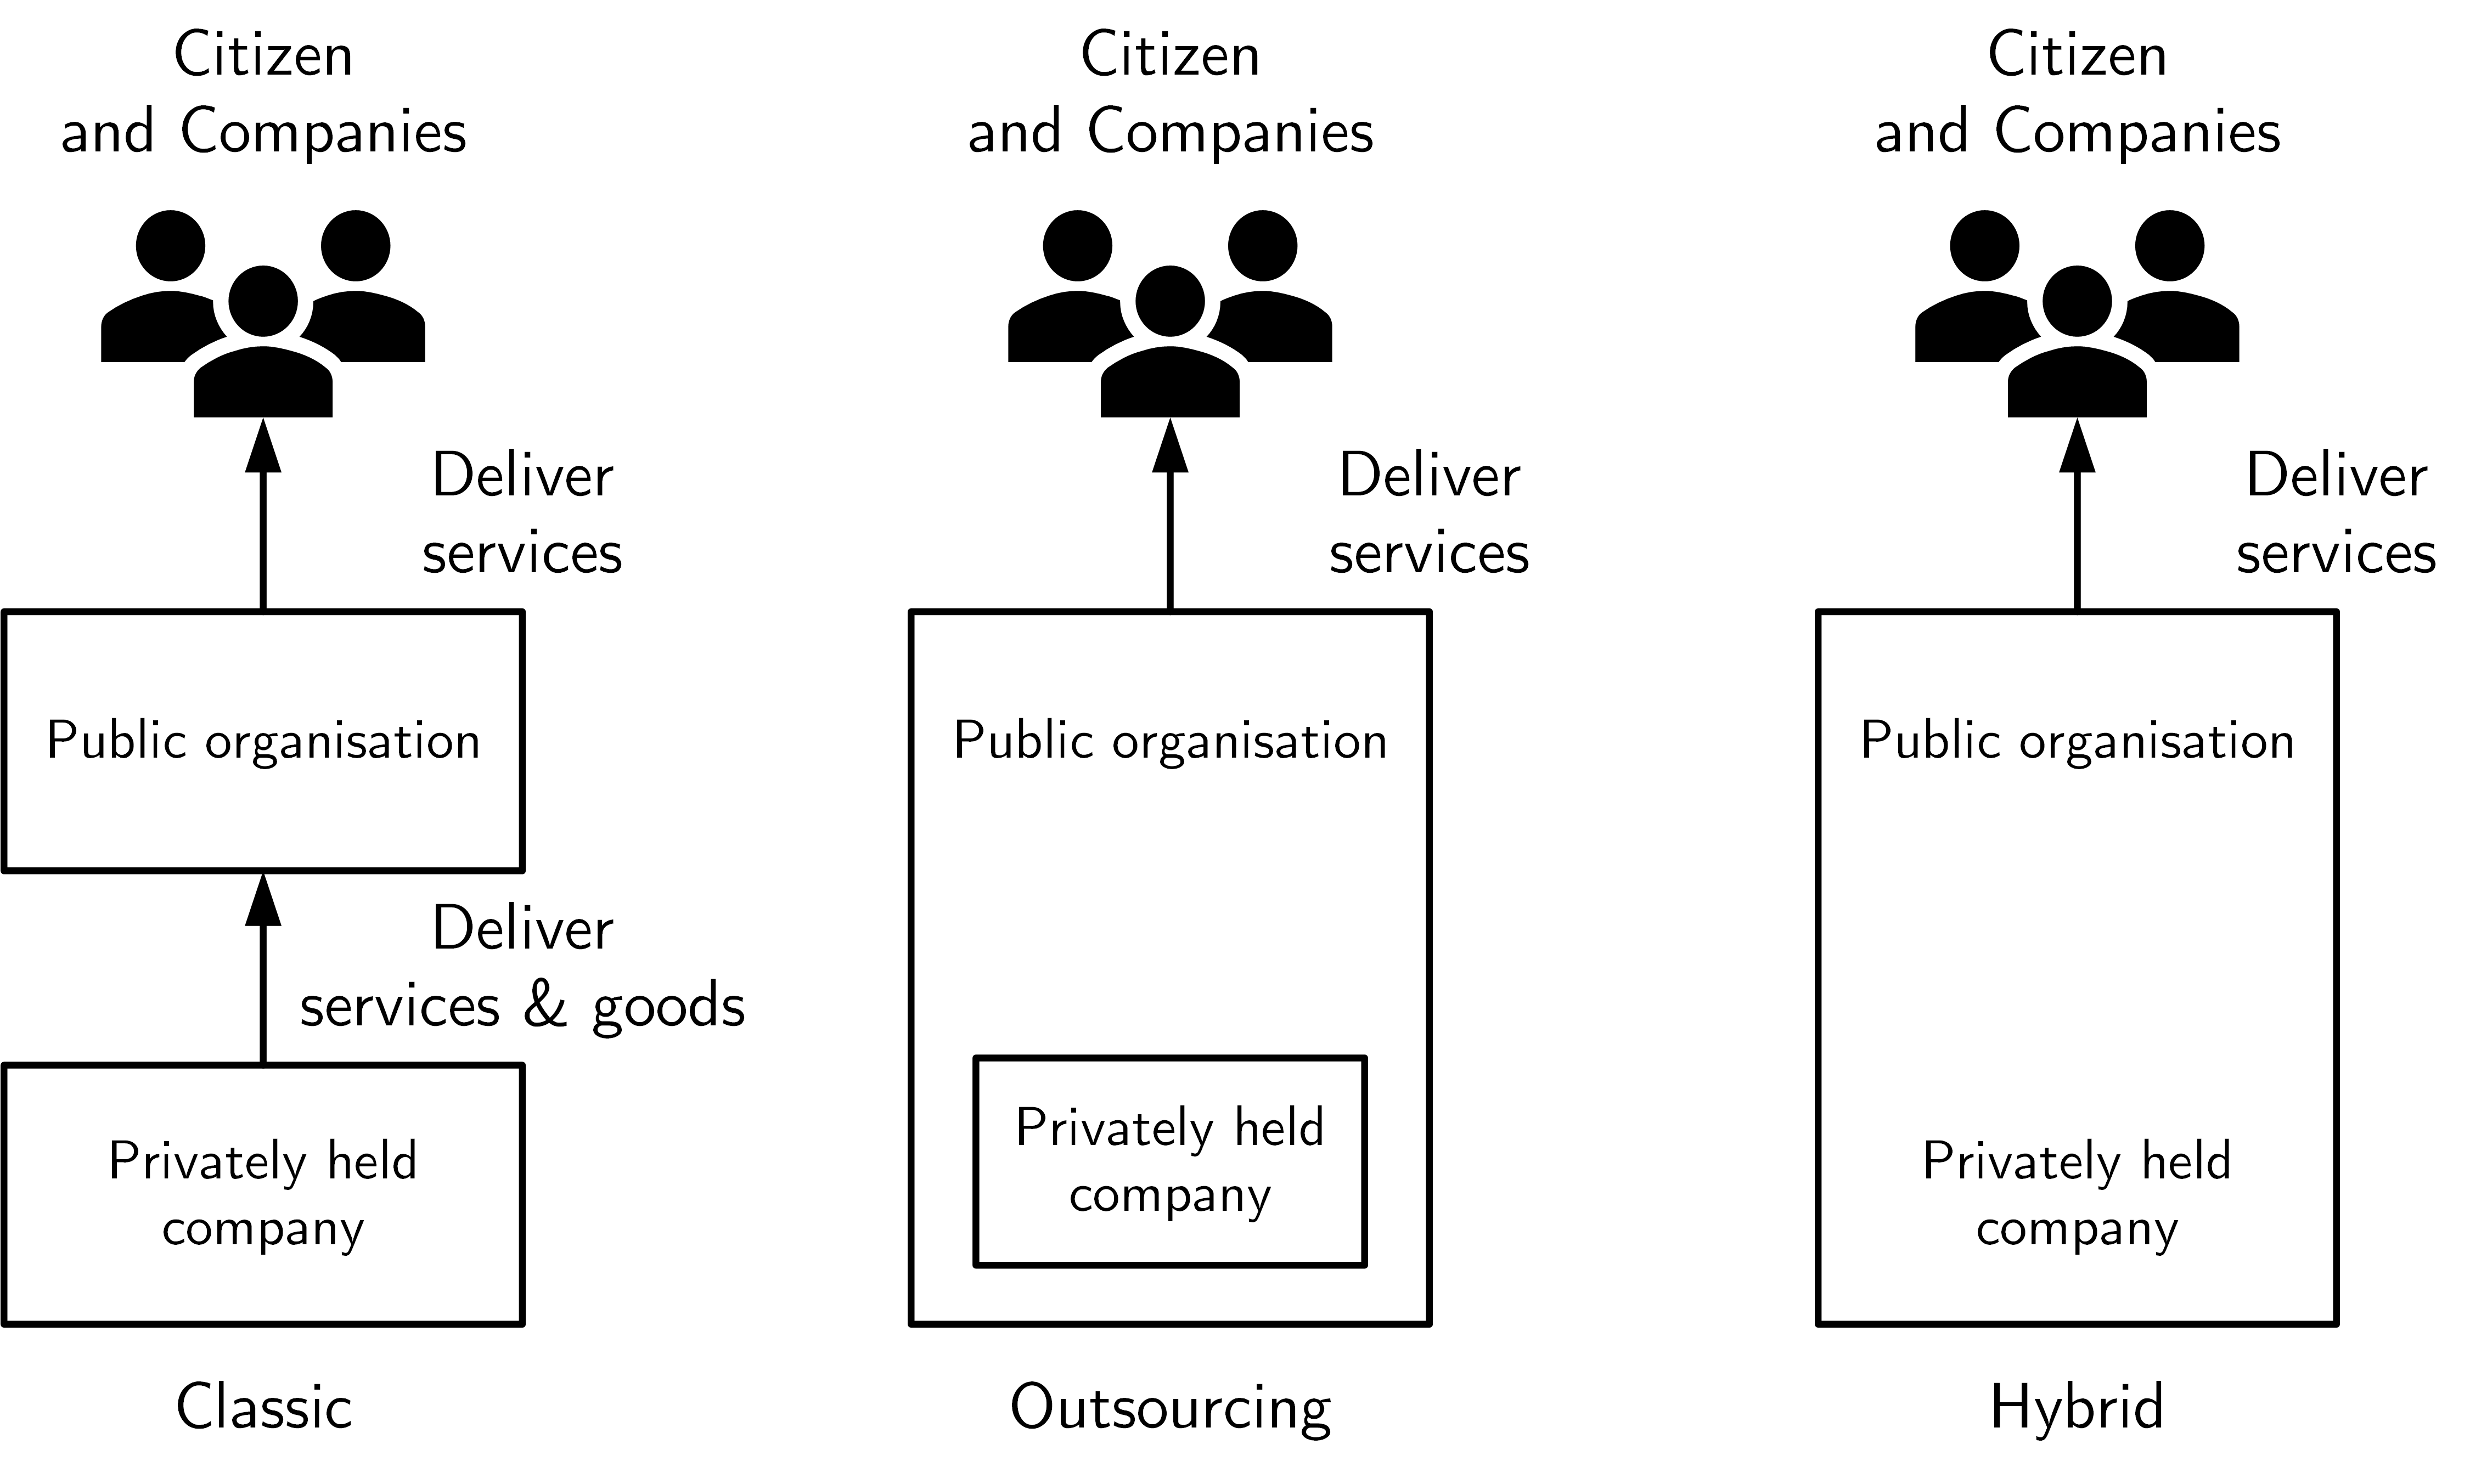
\includegraphics[width=0.7\linewidth]{images/publicsector3modelsofcolaboration}
	\caption[Public sector collaboration models]{Public sector collaboration models}
	\label{fig:publicsector3modelsofcolaboration}
\end{figure}

The public sector is divided into three levels \parencite{PrivacySense2016}:

\begin{itemize}
	\item{\textbf{The national government,} such as the military, the tax authority, and homeland affairs.}
	\item{\textbf{The regional government,} such as the provinces, the police, and water management.}
	\item{\textbf{The local government,} such as the municipalities, the social services, and the local tax offices.}
\end{itemize}

I will focus this research on the public sector level local government of the Netherlands. In \cref{ch:discussion} I will discuss the applicability on non Dutch public sectors.

\section{Introduction of the concept Enterprise Architecture}
\label{introea}
\acrfull{ea} is a discipline for proactively and holistically leading enterprise responses to disruptive forces by identifying and analysing the execution of change toward desired business vision and outcomes. \acrshort{ea} delivers value by presenting business and IT leaders with signature-ready recommendations for adjusting policies and projects to achieve targeted business outcomes that capitalise on relevant business disruptions \parencite{Gartner}.

\textcite{White2018} states that the organisation’s business requirements guide \acrshort{ea} — it helps layout how information, business and technology flow together. \acrshort{ea} has become a priority for businesses trying to keep up with new technologies such as the cloud, \acrfull{iot}, machine learning and other emerging trends that will prompt digital transformation.

IEEE Definition

Concept architectures needed for the problem statement (business, application, information, technology).

\section{Introduction of the concept of antifragility}
\label{sec:introantifragility}
\textcite{Taleb2008} describes a black swan as an event that 1) is so rare that even the possibility that it might occur is unknown, 2) has a catastrophic impact when it does occur, and 3) is explained in hindsight as if it were actually predictable. For extremely rare events, \citeauthor{Taleb2008} argues that the standard tools of probability and prediction, such as the normal distribution, do not apply since they depend on large population and past sample sizes that are never available for rare events by definition. Extrapolating, using statistics based on observations of past events is not helpful for predicting black swans, and might even make us more vulnerable to them. In his book \Gls{antifragile}, \textcite{Taleb2012} states that the way to survive a black swan event is to be \gls{antifragile}.\par
Most people answer that the opposite of \gls{fragile} is \gls{robust}, \gls{resilient}, solid, or something of the sort. However, the \gls{resilient}, \gls{robust} (and company) are items that neither break nor improve, so you would not need to write anything on them — have you ever seen a package with \gls{robust} in thick green letters stamped on it? Logically, the exact opposite of a \gls{fragile} parcel would be a package on which one has written, please mishandle or please handle carelessly. Its contents would not just be unbreakable but would benefit from shocks and a wide array of trauma \parencite{Taleb2012}.

\begin{figure}[h!]
	\centering
	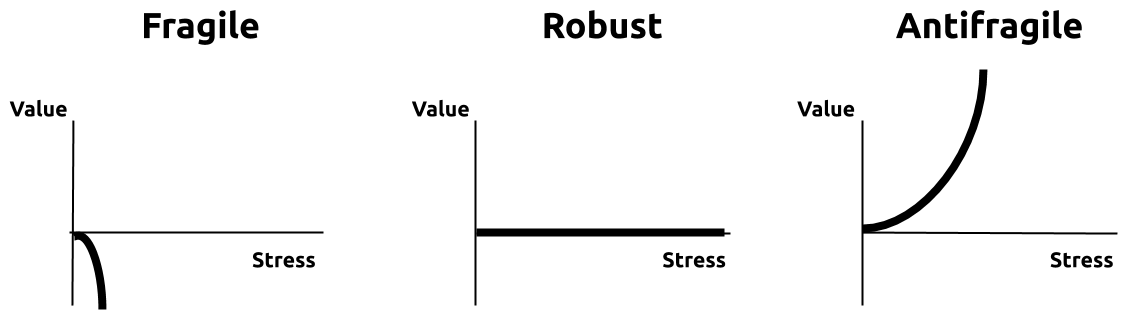
\includegraphics[width=0.7\linewidth]{images/eaal-triad}
	\caption[EAAL Triad]{\acrshort{eaal} Triad \parencite{Botjes2020}}
	\label{fig:eaal-triad}
\end{figure}

\section{Problem statement}
\label{sec:problemstatement}
The concept of \gls{antifragility} implies that organisations could benefit and strengthen from crises, volatility, errors and uncertainty and could also lead to opportunities for innovation \parencite{Kastner2017}. Enterprise Architecture is a discipline that helps organisations to reach their goals. As stated by 

As described in \ref{introea} with \acrshort{ea} one would expect that an organisation uses the discipline of \acrshort{ea} to get more towards the state of \gls{antifragility}. Research has been conducted on aspect architectures such as the application and information architectures but not on \acrshort{ea}. The problem is that the Body of Knowledge contains no direct knowledge on how to achieve \gls{antifragility} with the use of \acrshort{ea}. 

\section{The research subject}
\label{sec:researchsubject}
\acrshort{ea} facilitates an organisation in assessing the impact of change and making recommendations for target states that support business objectives. \acrshort{ea} guides an organisation in changing. \acrshort{ea} can help organisations in changing towards the state of \gls{antifragility}.

As described in \ref{introea} \acrshort{ea} is used to steer an system towards its goals. However, what are the success factors of \acrshort{ea} that contribute in accomplishing \gls{antifragility}? This is summarised in a conceptual research model.
\begin{figure}[H]
	\centering
	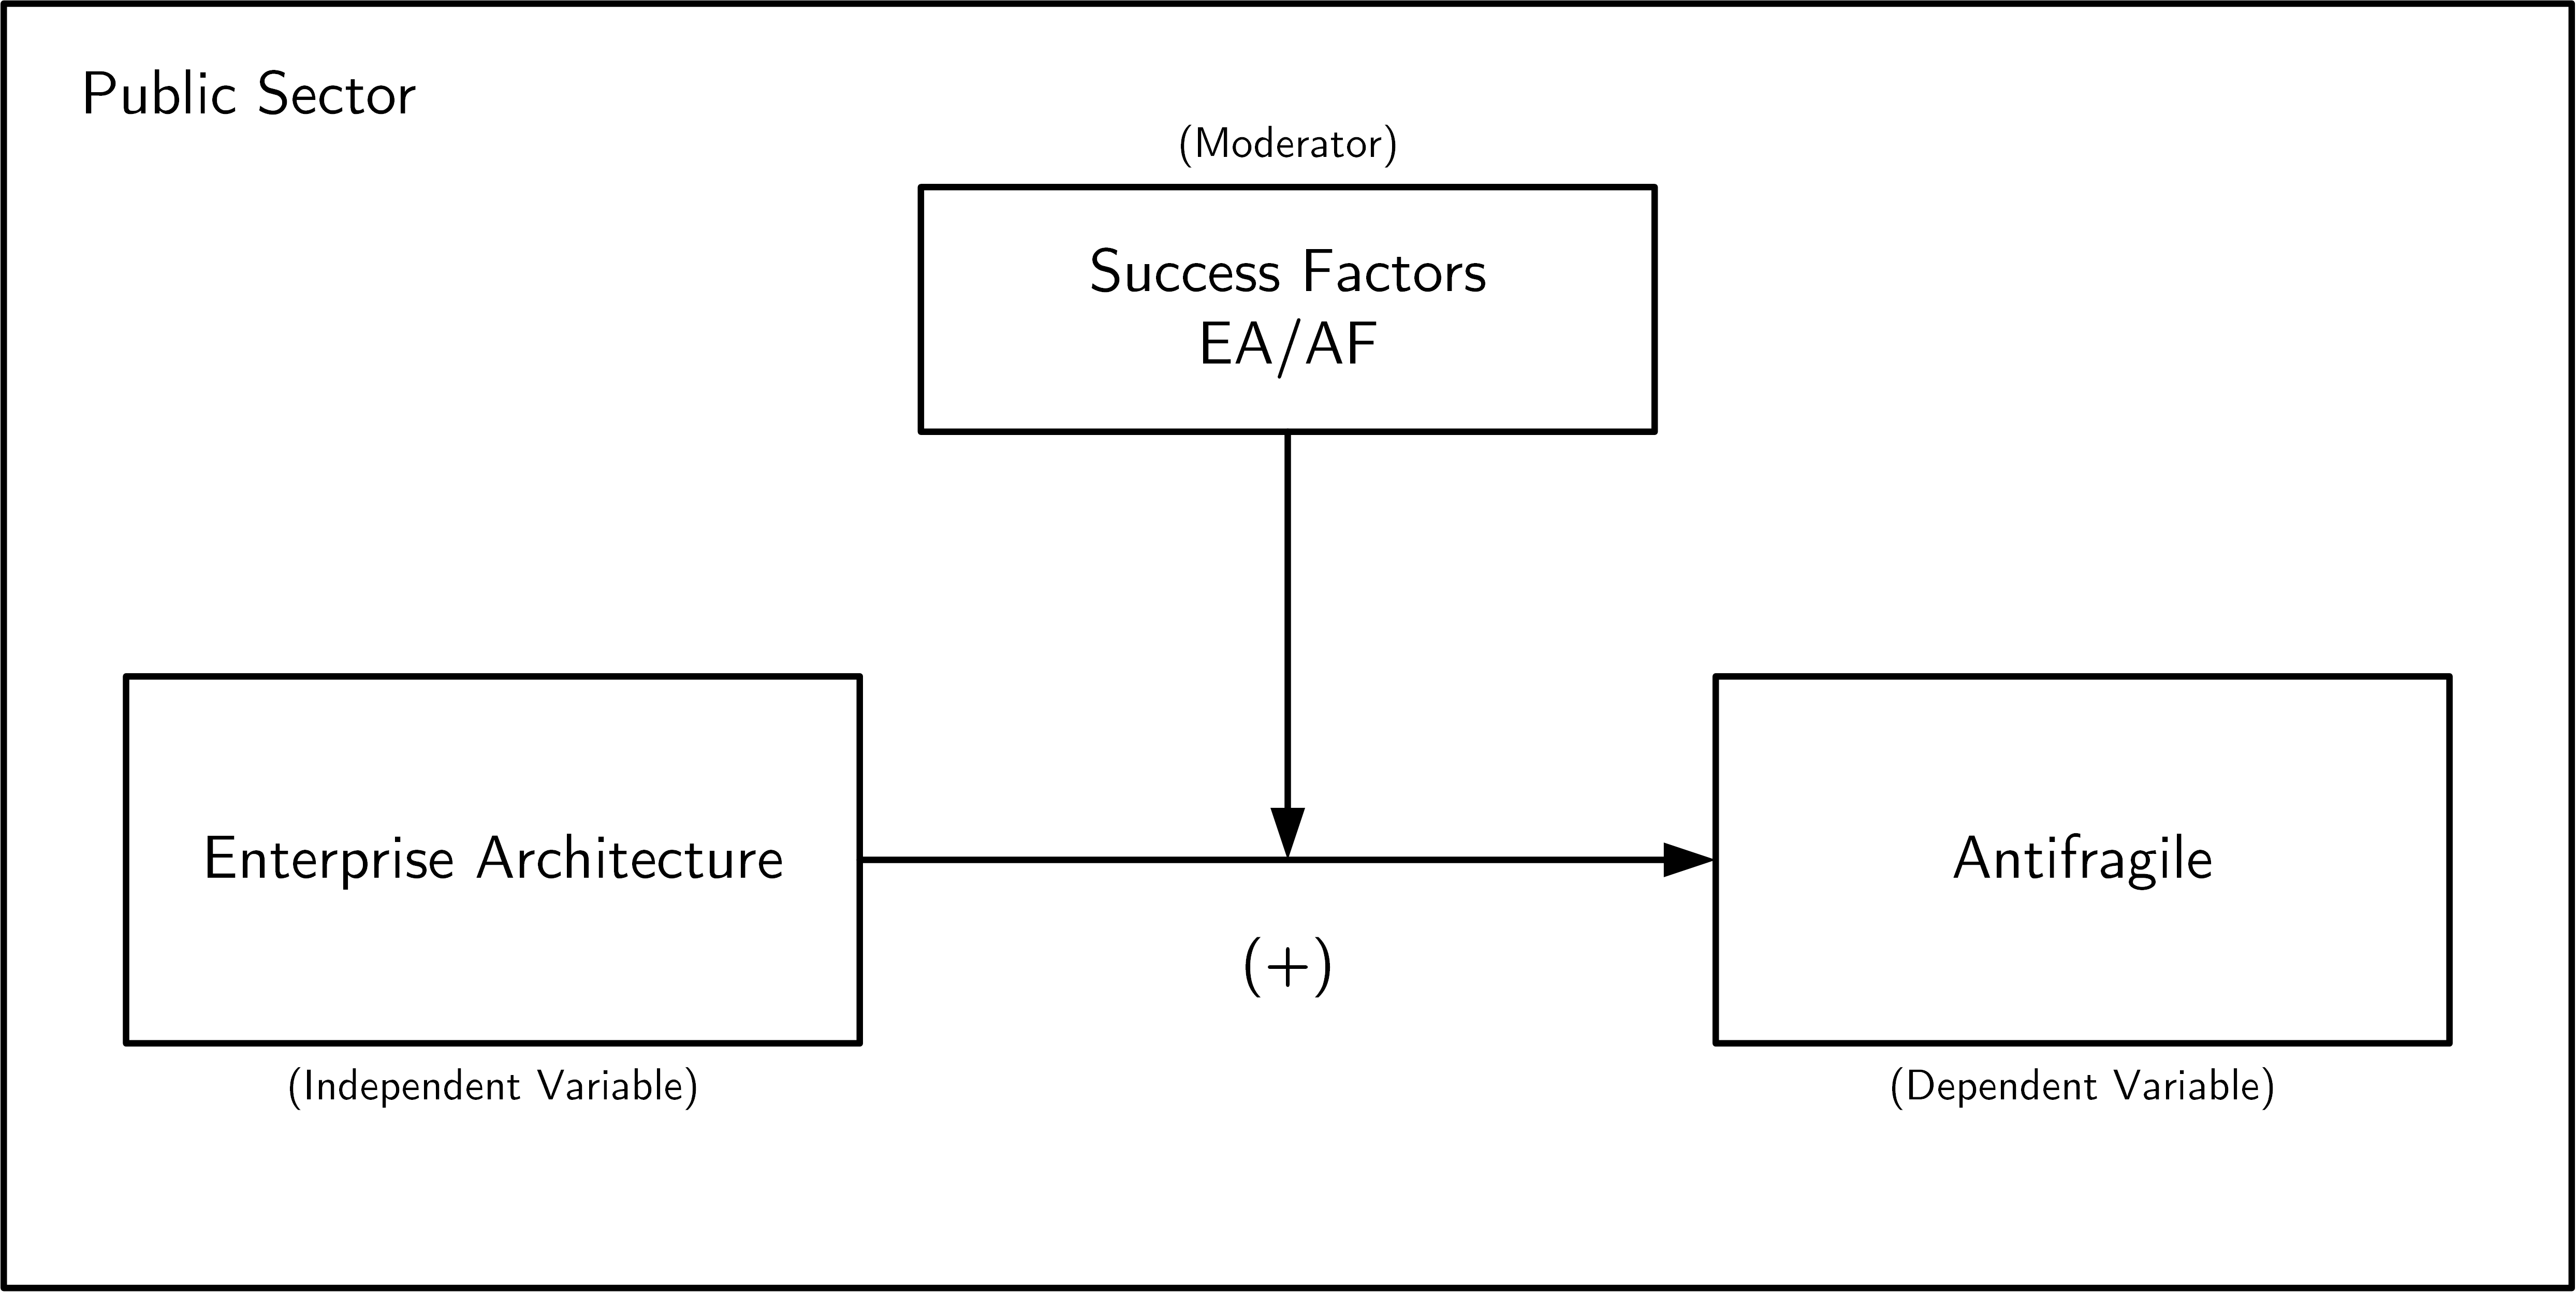
\includegraphics[width=0.8\linewidth]{images/conceptualmodel}
	\caption[Conceptual Research Model]{Conceptual Research Model}
	\label{fig:conceptualmodel}
\end{figure}

The hypothesis of the conceptual research model is that, in the context of the system public sector, \acrlong{ea} success factors have a positive influence in the contribution of \acrlong{ea} in achieving antifragility in that system. From this conceptual research model the research question can be stated as:\bigskip

\noindent \emph{''What are the success factors of \acrlong{ea} for \gls{antifragility} in the public sector?''}\bigskip

\noindent To correctly answer this research question the following sub-questions need to be answered:

\begin{enumerate}
	\item{What is literature saying about the public sector?}
	\item{What is literature saying about \acrlong{ea}?}
	\item{What is literature saying about the success factors of Enterprise Architecture?}
	\item{What does literature say about antifragile?}
%	\item{How can the success factors of \acrlong{ea} contribute to becoming antifragile?}
\end{enumerate}
\section{Research relevance}
\label{sec:researchrelevance}

\acrfull{ea} has contributed to being more \gls{robust}, \gls{resilient}, and \gls{agile}. Using \acrshort{ea} in pursuing \gls{antifragility} will add value to companies by accelerating and growing when there is a stressor or black swan event. The \gls{antifragile} theory is young.  \citeauthor{Taleb2012} published the theory in his book ''\Gls{antifragile}: Things that gain from disorder.'' in \citeyear{Taleb2012}.  Studies conducted on \acrshort{ea} with the concept of \gls{antifragile} are almost non-existence. The conducted studies are primarily about making IT Systems \gls{antifragile}. \textcite{Botjes2020,Kastner2017} are exceptions and have researched how to apply \gls{antifragile} in an organisational context. Nevertheless, both concluded that there is more research needed. The former used the lens of Enterprise Engineering, which is closely related to \acrshort{ea}, together with resilience, while the latter used mostly reslience as its lens. There is still no answer to how \acrshort{ea} can contribute to becoming \gls{antifragile}. Organisations use the practice of \acrshort{ea} to guide them to achieve their goals. Giving more insights on this subject will contribute to the Body of Knowledge and help others getting closer to \gls{antifragility} by using \acrshort{ea}.

\begin{figure}[H]
	\centering
	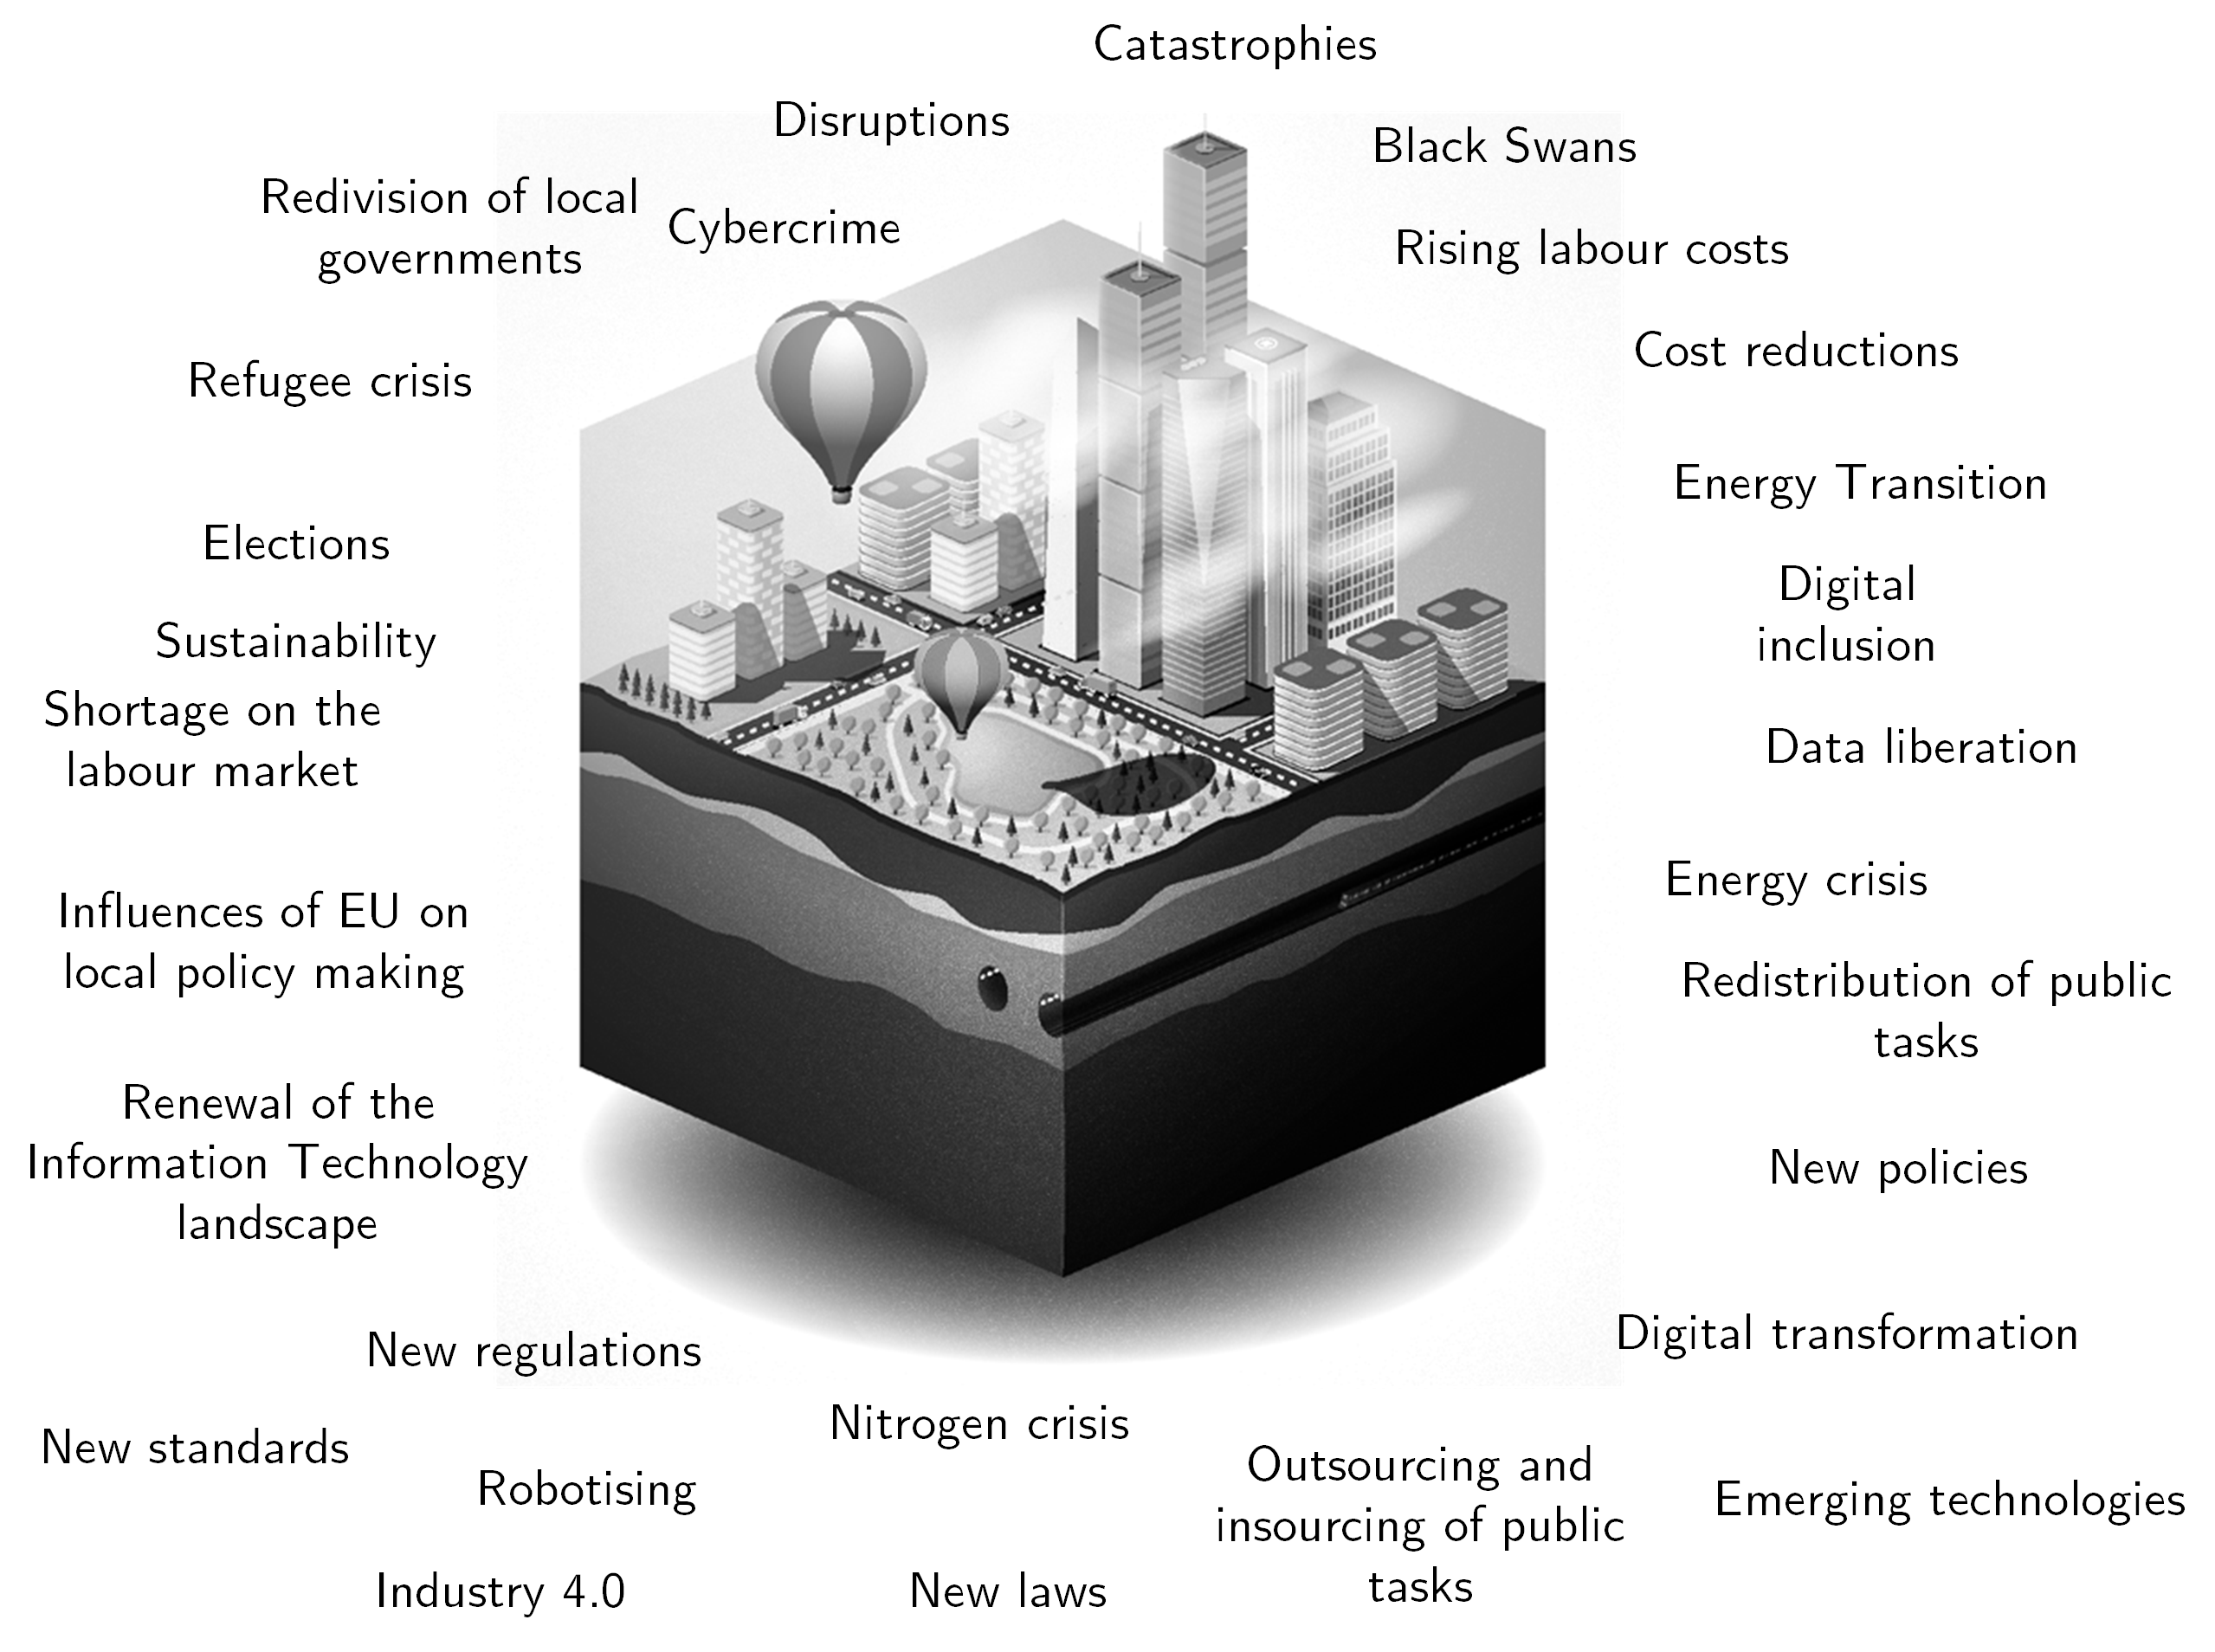
\includegraphics[width=0.8\linewidth]{images/publicstressors}
	\caption[Examples of stressors on the public sector (local governments)]{Examples of stressors on the public sector (local governments)}
	\label{fig:publicstressors}
\end{figure}

Because of the digital transformation, the pace of change is increasing rapidly.  The digital transformation is not the only stressor on the public sector. There are a lot of internal and external stressors. The public sector invested a lot in being less fragile by becoming more agile, robust, and resilient. By being more agile, robust, or resilient, you can only withstand the change or the stressor but you do not gain from it. Governmental agencies and suppliers in the public sector are searching for methods of dealing with this increased pace and the disruptions that occur. The relevance of this research is not only about the addition to the Body of Knowledge but also to share the outcome with the public sector.

 %	Add the introduction
	
	\chapter{Research Methodology}
\label{ch:research-methodology}

\section{Research Model}
\label{sec:research-model}
The method of \textcite{Verschuren2016} is used for the research model. This method gives me a step-by-step plan for the research.
	\begin{figure}[h]
		\centering
		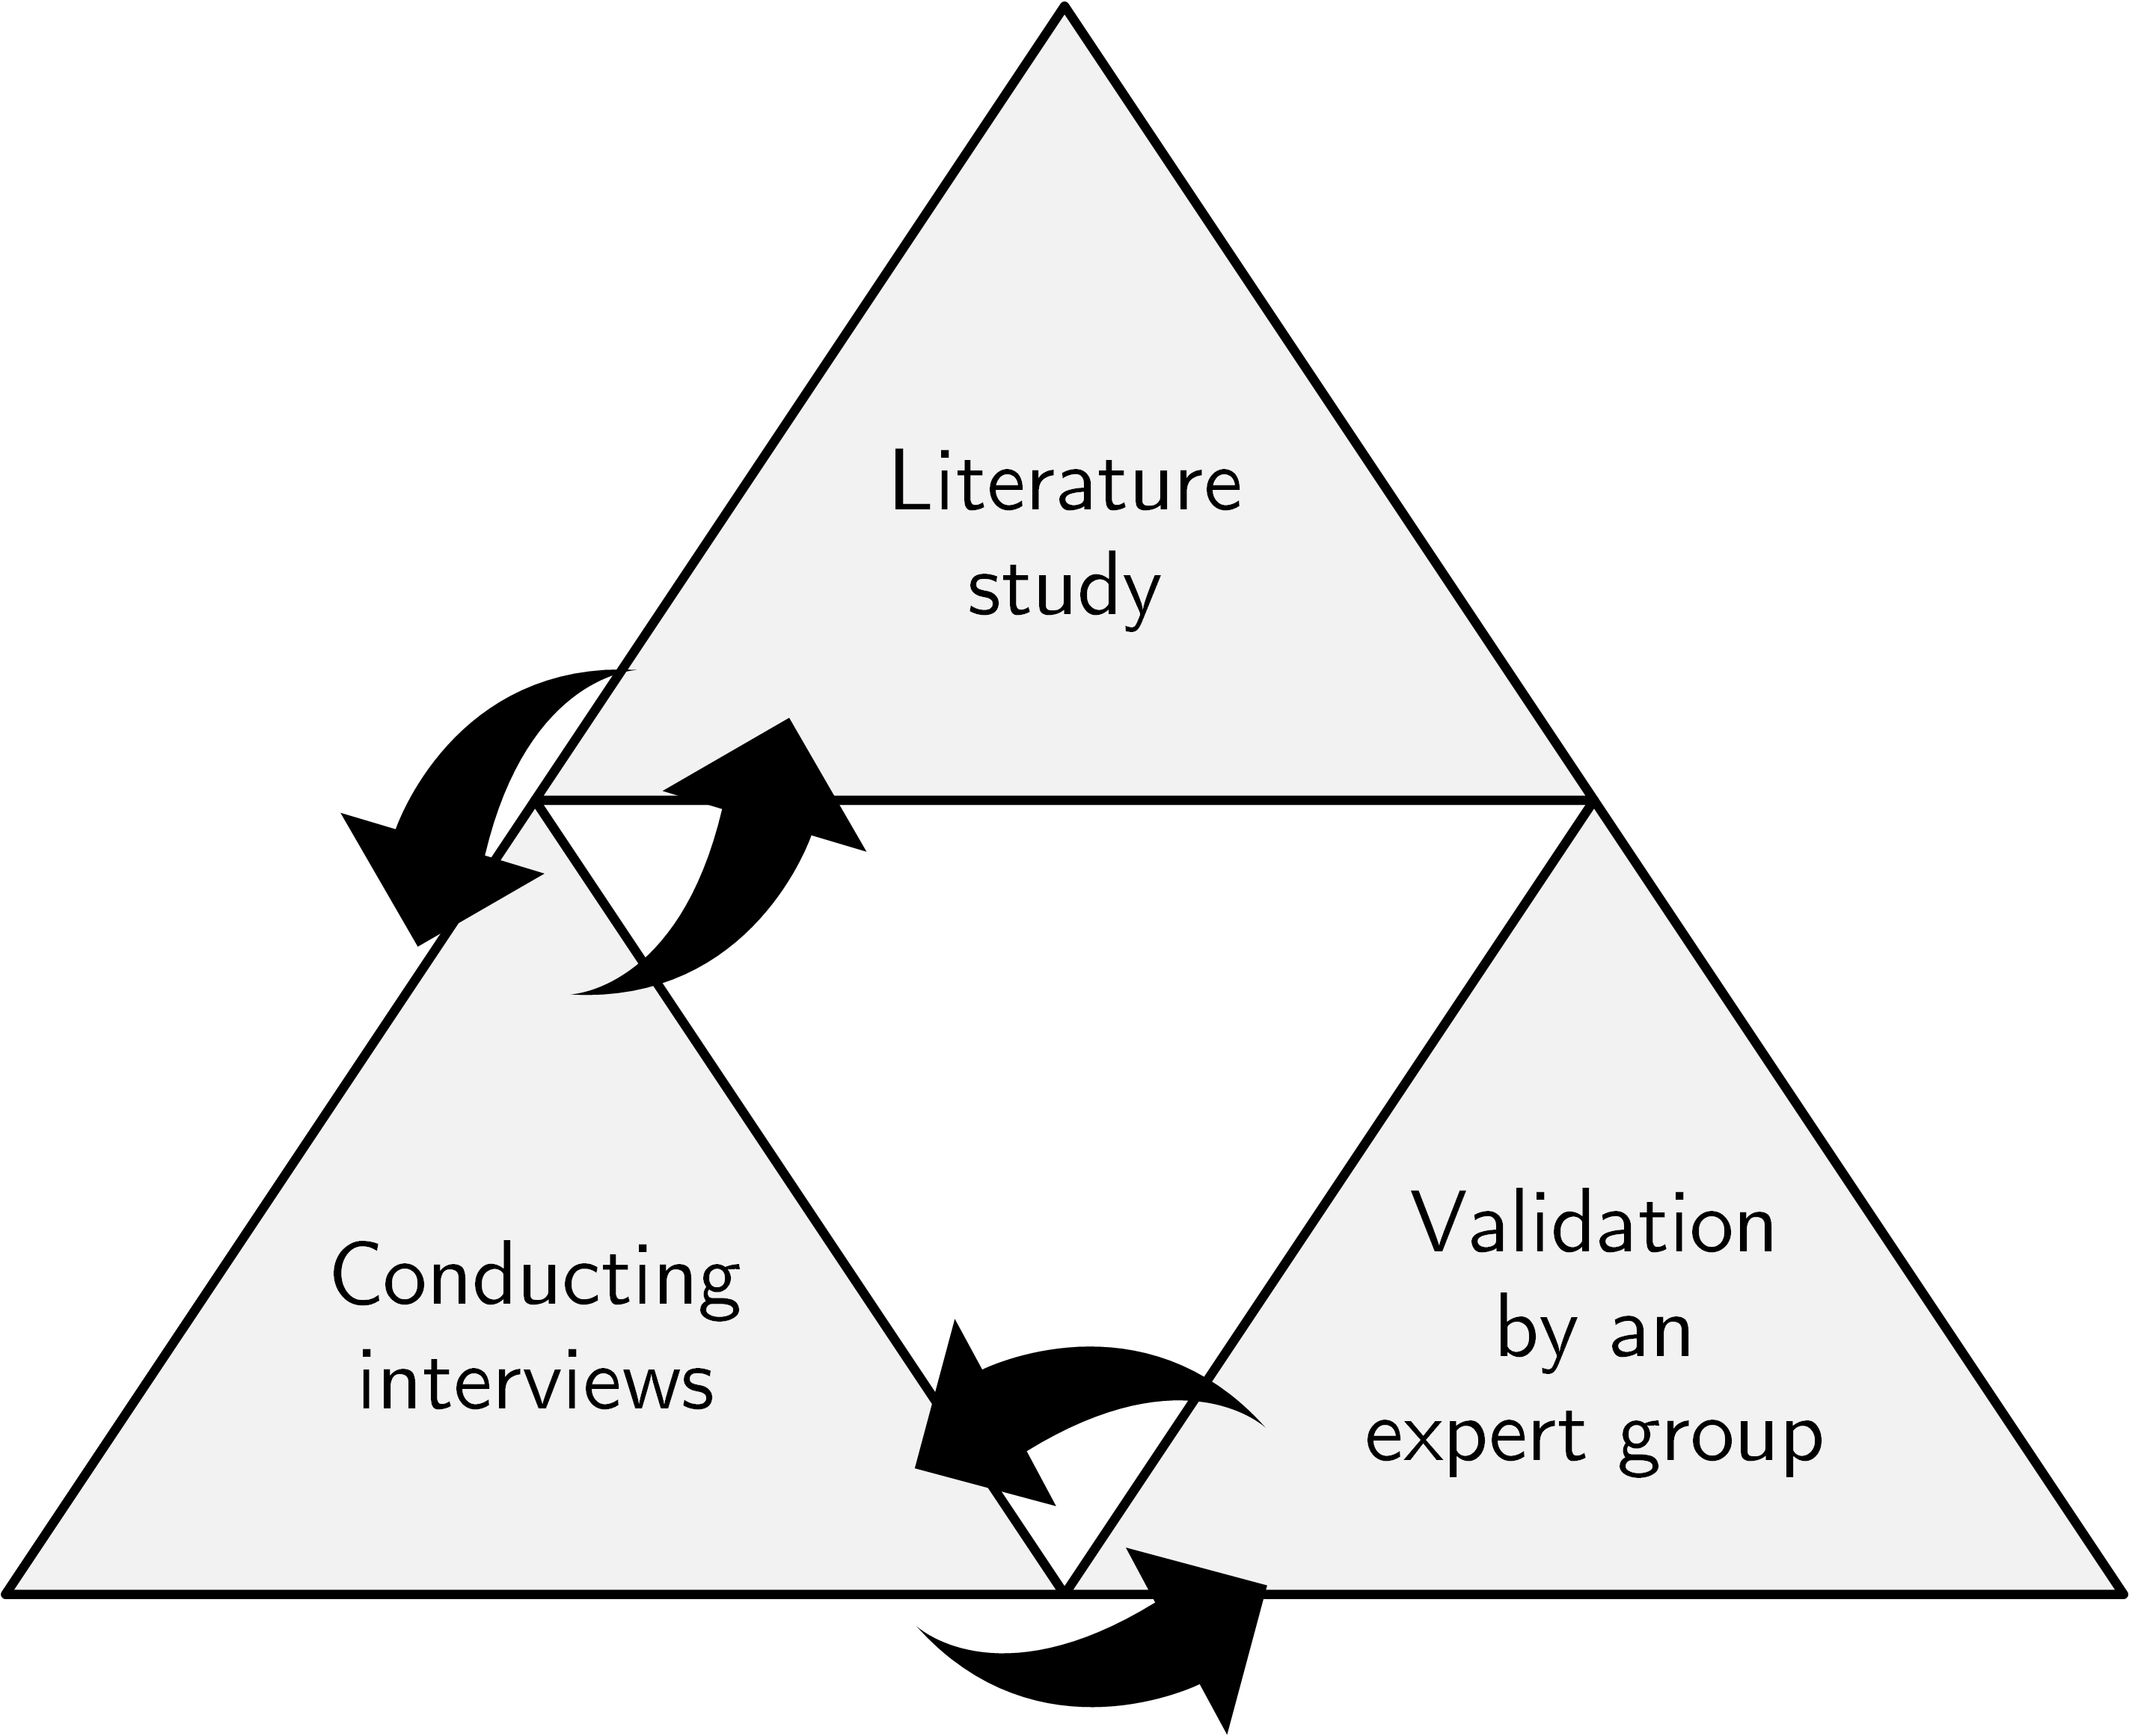
\includegraphics[width=14cm]{images/researchmodel.png}
		\caption[Research Model]{Research Model}
		\label{fig:research-model}
	\end{figure}

In the first phase of research (a), I conduct preliminary research and I study different theories and definitions of the involved concepts. The output of the first phase is the definitions and theories relevant to this research, such as \gls{antifragile}, \acrlong{ea}, the public Ssctor market, and \acrshort{vuca}. In the second phase of research (b), I confront \gls{antifragile} with \acrlong{ea} and the public sector market with \acrshort{vuca}. I am using interviews to validate the confrontation between the public sector Market with \acrshort{vuca}. The outcome of the second phase is the initiation of analysis on success factors of \acrlong{ea} relevant for contribution to \gls{antifragile} and analysis on attributes of the public sector market influenced by \acrshort{vuca} (c). In the fourth phase (d), I used the output of the analysis to confront the success factors with a Delphi Group for validation through the Delphi Method to conclude and discuss his research (e).

\begin{remark}
	Missing the outcome of the confrontation of (a) that is used by all concepts in (b).
\end{remark}
\section{Research quality}
\label{sec:researchquality}
I use three frameworks to guide me to increase the rigorousness of the research.
\begin{itemize}
	\item{Quality Principles of \textcite{Recker2013} (subsection \ref{sub:recker}).}
	\item{The FAIR Principles from Scientific Data (subsection \ref{sub:fair}).}
	\item{The Open Science Framework (subsection \ref{sub:osf}).}
\end{itemize}
\subsection{Quality Principles of Recker}
\label{sub:recker}
The first framework is that of \textcite[p. 16-17]{Recker2013} who uses four important principles:
\begin{itemize}
	\item{\textbf{Replicability} is a term that characterises the extent to which research procedures are repeatable. The principle states that the procedures by which research outputs are created should be conducted and documented in a manner that allows others outside the research team to independently repeat the procedures and obtain similar, if not identical, results.}
	\item{\textbf{Independence} is closely related to reliability. It concerns the extent to which the research conduct is impartial and freed from any subjective judgment or other bias stemming from the researcher or research team itself.}
	\item{\textbf{Precision} states that in all scientific research the concepts, constructs, and measurements should be as carefully and precisely defined as possible to allow others to use, apply, and challenge the definitions, concepts, and results in their own work.}
	\item{\textbf{Falsification} describes the logical possibility than an assertion, hypothesis, or theory can be contradicted by an observation or other outcome of a scientific study or experiment.}
\end{itemize}
\begin{remark}
	Howto falsify? 
\end{remark}
\subsection{Fair Principles}
\label{sub:fair}
In 2016, the 'FAIR Guiding Principles for scientific data management and stewardship' were published in Scientific Data. The authors intended to provide guidelines to improve the Findability, Accessibility, Interoperability, and Reuse of digital assets. The research is using the FAIR Principles\footnote{\url{https://www.go-fair.org/fair-principles/}} to increase the quality of the published thesis.
\begin{itemize}
	\item{\textbf{Findable.} The first step in (re)using data is to find them. Metadata and data should be easy to find for both humans and computers. Machine-readable metadata are essential for automatic discovery of datasets and services. The thesis, research and used datasets are containing keywords, links, and structures that can be indexed.}
	\item{\textbf{Accesible.} Once the user finds the required data, she/he/they need to know how can they be accessed. The thesis, research and used datasets are published on GitHub, Zenodo, and Researchgate based on Open Access. I create objects containing a location on where the data can be acquired if it cannot be published because of author rights.}
	\item{\textbf{Interoperable.} The data usually need to be integrated with other data. In addition, the data need to interoperate with applications or workflows for analysis, storage, and processing. This principle is not relevant for this research. The data are qualitative data sets based on literature, interviews, and questionnaires.}
	\item{\textbf{Reusable.} The ultimate goal of FAIR is to optimise the reuse of data. To achieve this, metadata and data should be well-described so that they can be replicated and/or combined in different settings. The thesis, research and used datasets are published under the \href{https://creativecommons.org/licenses/by-sa/4.0/}{\ccbysa\ CC-BY-SA 4.0 license.} It is allowed that the thesis, research, and datasets are shared and are adapted (even commercially) as long as the original author is attributed and the possible derivate is published under the same license.}
\end{itemize}
\subsection{The Open Science Framework}
\label{sub:osf}
One of the starting points of the research is Open Science. The idea behind Open Science is to allow scientific information, data and outputs to be more widely accessible (Open Access) and more reliably harnessed (Open Data) with the active engagement of all the stakeholders (Open to Society) \parencite{UNESCO2020}. The Center for Open Science\footnote{{\url{https://www.cos.io/}}} supports this way of research by supplying guidelines and even a toolkit. For this research the toolkit is used to support Open Access, Open Data and Open to Society. One of the tools in the toolkit is a reference model to select tools for the four main phases of research: Search and Discover, Design Study, Collect and Analyse Data, and Publish Reports. I use this reference model in section \ref{sec:researchinfraandtooling}. Using this framework will help in achieving replicability, precision, and reusability.
\section{Research approach}
\label{sec:researchapproach}
In this section, I describe the approach of the research. This description helps to increase replicability, independence, and reusability. For this research approach, I follow the research model (figure \ref{fig:research-model}) and the research (sub)questions (section \ref{sec:researchsubject}). The research model contains five phases in the research. The five phases are used to describe the research approach. The five phases are (a) Desk research, (b) Confrontation, (c) Analysis, (d) Validation, and (e) Conclusion and discussions.

\subsection{Desk research}
\label{sub:deskresearchphase}
The first phase of the research model emphasises desk research on the relevant concepts, theories and definitions. Desk research is conducted based on a literature study. The main concepts of \gls{antifragile}, \acrshort{ea}, \acrshort{vuca}, and the public sector are studied. This first phase (a) will answer the sub-questions of:
\begin{itemize}
	\item{What is literature saying about \gls{antifragile}?}
	\item{What is literature saying about the public sector?}
	\item{What is literature saying about \acrlong{ea}?}
	\item{What is literature saying about the success factors of Enterprise Architecture?}
\end{itemize}

\subsubsection{Literature research}
For the literature research two primary methods are used. The first method is (foward and backward) snowballing of already acquired literature. The second method is the use of online scientific libraries.

\begin{figure}[H]
	\centering
	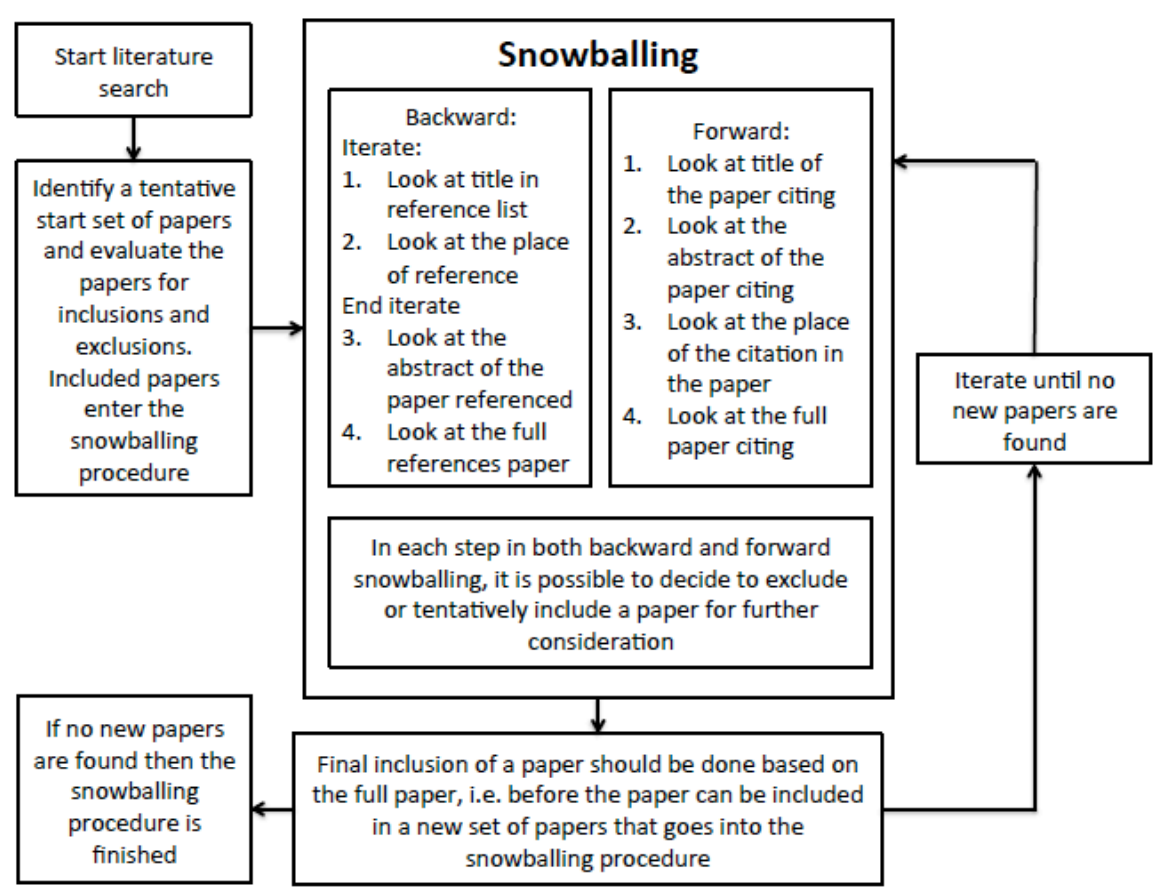
\includegraphics[width=0.6\linewidth]{images/snowball}
	\caption[Snowballing literature]{Snowballing literature \parencite{Botjes2021a}}
	\label{fig:snowball}
\end{figure}

For finding relevant literature online scientific libraries are used. The online scientific libraries are Web of Science, Research Gate, and Google Scholar. The full concept name is used and the known abbreviations of the concept (e.g. Enterprise Architecture and EA). The list of abbreviations contains the used abbreviations. Literature is only accepted if the literature complies with quality attributes. These attributes are accuracy, authority, objectivity, currency, and coverage\footnote{\url{https://libguides.library.cityu.edu.hk/litreview/evaluating-sources/}}. All found literature is administrated for replicability, independence, precision, accessibility, and reusability. Section \ref{sub:tbresearchexecution} describes how literature registration and administration is executed.

\subsubsection{Antifragile}
\label{subsub:antifragile}
The literature study on \gls{antifragile} makes use of four primary sources. The first primary source is the book ''\Gls{antifragile}: Things that gain from disorder'' \parencite{Taleb2012}. \textcite{Taleb2012} is the progenitor of the \gls{antifragile} theory. The second primary source is the master thesis ''Defining \Gls{antifragility} and the application on Organisation Design" \parencite{Botjes2020}. \citeauthor{Botjes2020} studied the literature, extensively, in the field of \gls{antifragile} and the application in the context of an organisation. By using the thesis of \citeauthor{Botjes2020} the literature study of this study concentrates on the literature after 2018. The last two primary resources are the articles ''No More Snake Oil: Architecting \Gls{agility} through \Gls{antifragility}'' and ''The Philosophy of Residuality Theory'' \parencite{OReilly2019,OReilly2021}. \textcite{Botjes2020} did not use the articles of \citeauthor{OReilly2019}. The theories of \citeauthor{OReilly2019} were less of interest for the subject of \citeauthor{Botjes2020}. While for this research the Residuality Theory of \textcite{OReilly2021} has added value since it targets system architecture.

\begin{remark}
	Need to add second book from Taleb (Black Swan) since Antifragile is an answer to black swan events.\\
	Need to add book of Hole as it is one of the sources referenced by many.
\end{remark}

The first method for literature study is snowballing. Snowballing of these sources is used to determine other important literature on \gls{antifragile}. Forward snowballing is used for the source of \citeauthor{Taleb2012}. Since \citeauthor{Taleb2012} is the progenitor, it is not necessary to do a backward snowballing. Backward snowballing is used for the sources from \citeauthor{Botjes2020} and \citeauthor{OReilly2019}.

The second method for literature study is the use of online scientific libraries. For these libraries the following set of keywords or key sentences are used.
\bigskip

\begin{table}[H]
	\centering
\begin{tabular}{p{0.4\textwidth}p{0.4\textwidth}}
	\toprule
	\gls{antifragile}	& \gls{antifragile} \gls{robust} \gls{resilient} \gls{agile}\\%
	\gls{antifragile} \acrlong{ea}	& \gls{antifragile} public sector\\%
	\gls{antifragile} success factors & residuality theory\\%
	\gls{antifragile} residuality theory & \acrlong{vuca} \\%
	\gls{antifragile} system & \\%
	\bottomrule
\end{tabular}
	\caption{Antifragile keywords}
\end{table}

\subsubsection{Enterprise Architecture}
\label{subsub:enterprisearchitecture}
The literature study on \acrshort{ea} makes use of three primary sources. \textcite{Greefhorst2011} is a book on the theory on steering mechanisms of \acrshort{ea} with the emphasis on the use of principles. \textcite{Ross2014} is the most referenced book on the subject \acrshort{ea} and Business Strategy. The last one is the article of \textcite{Lapalme2012} who researched the different manifestations of \acrshort{ea}.

The first method is snowballing. All three sources will be used for forward and backward snowballing. The second method for literature study is the use of online scientific libraries. For these libraries the following set of keywords and key sentences are used:
\bigskip

\begin{table}[H]
	\centering
\begin{tabular}{p{0.4\textwidth}p{0.4\textwidth}}
	\toprule
	\acrlong{ea} & \acrlong{ea} sucess factors\\%
	\acrlong{ea} \gls{antifragile} system	& \acrlong{ea} steering mechanism\\%
	intentional emergent \acrlong{ea} & \acrlong{ea} Business Strategy\\%
	\acrlong{ea} public sector & \\%
	\bottomrule
\end{tabular}
	\caption{Enterprise Architecture keywords}
\end{table}

\subsubsection{Public sector}
\label{subsub:publicsector}
The literature study on public sector makes use of one primary source. \textcite{Wal2008} is an article on the differences between the public and private sector based on the core values of these sectors. This article is used for forward and backward snowballing. The last method for literature study is the use of online scientific libraries. For these libraries the following set of keywords and key sentences are used:
\bigskip

\begin{table}[H]
	\centering
	\begin{tabular}{p{0.4\textwidth}p{0.4\textwidth}}
		\toprule
		Difference public and private sector &	public sector \gls{antifragile}\\%
		Collaboration public and private sector & public sector \gls{resilient}\\%
		public sector \acrshort{vuca} & \\%
		\bottomrule
	\end{tabular}
	\caption{Public sector keywords}
\end{table}

\begin{remark}
	The preliminary research on the topic public sector is not started yet. Maybe some primary sources will emerge.
\end{remark}

\subsection{Confrontation}
\label{sub:confrontationphase}

For the confrontation of VUCA with the public sector interviews are used to....\\
For the confrontation of EA with EA a framework/model is needed! (part of Theoretical background)

\begin{remark}
	What is the model for confrontation?
	I have to determine the lens I am going to use.
\end{remark}

The second phase (b) 

\subsection{Analysis}
\label{sub:analysisphase}

\begin{remark}
	What is the model for Analysis?
	I have to determine the lens I am going to use.
\end{remark}

The third phase (c)

How can the success factors of \acrlong{ea} contribute to becoming antifragile?

\subsection{Validation}
\label{sub:validatinphase}
%The fourth phase (d) analyses the outcome of the analysis phase. This outcome is the answer to the sub-question ''How can the success factors of \acrlong{ea} contribute to becoming antifragile?'' 
The success factors are validated by the means of the Delphi Method.

\subsubsection{Delphi Method}
\label{subsub:delphimethod}
The Delphi method is an iterative process to collect and distil the anonymous judgments of experts using a series of data collection and analysis techniques interspersed with feedback. The Delphi method is well suited as a research instrument when incomplete knowledge about a problem or phenomenon. The Delphi method evolved into a flexible research method appropriate for many \acrfull{is} research projects, such as determining the criteria for \acrshort{is} prototyping decisions, ranking technology management issues in new product development projects, and developing a descriptive framework of knowledge manipulation
activities. The Delphi method is a flexible, effective and efficient research method that can be successfully used by \acrshort{is} graduate students to answer research questions in \acrshort{is} and to advance the \acrshort{is} Body of Knowledge rigorously. \parencite{Skulmoski2007}

The group participants are mutually unknown, I am the only one who knows who the participants are. When it cannot be proven that the artefact is incorrect, it must be correct. This method is the principle of falsification. To reach a consensus, I use questionnaires. To reach a consensus, I am working iterative and adjusts the artefact after the feedback. I expect consensus on the artefact after two to six rounds of questionnaires. The goal of the Delphi Rounds is that it cannot be proven that the sucess factors are incorrect. This method is the principle of falsification (subsection \ref{sub:recker}). However, when is there a consensus? \textcite[p. 404]{Diamond2014} concludes in his research for over more than 100 cases that the median of the percentage of consensus 75\% is. I state, as a result of the research of \textcite{Diamond2014}, that consensus is reached with the threshold of 75\%. I state with some degree of certainty that the artefact is correct with a consensus of 75\%.

I defined domains for the group composition based on the context of the research. These domains are \acrfull{isv}, Municipality, National Government, VNG-Realisatie (the association of Dutch municipalities), and Academics. Participants are members of one or more of these domains and have an affinity with Enterprise Architecture and the public sector. I invite at least three participants per domain (n=3). The result is a total population of at least fifteen (n=15). The approach followed \textcite{Denzin2017} multiple triangulation approach, which encourages several methods to collect data and multiple investigators with varied expertise.

For the Delphi Group composition domains are defined based on the context of the research. These domains are \acrfull{isv}, Municipality, National Government, VNG-Realisatie (the association of Dutch municipalities), and Academics. The participants have affinity with \acrshort{ea}. The participants validate the artefact their context and domain.

Meeting Wizard is the service for sending out the questionnaires and execute the analysis of the outcome of the questionnaires. The participants get an invite by email to fill in the questionnaires. I analyse the results after every round and communicates the outcome as soon as a consensus is reached.

\subsection{Conclusion and discussion phase}
\label{sub:conclusionanddiscussinophase}
The fifth phase (e)

What are the success factors of \acrlong{ea} for \gls{antifragility} in the public Sector?

\section{Research type}

\begin{remark}
	Qualitative vs Quantitative! (use \parencite{Recker2013})
\end{remark}


\section{Research infrastructure and tooling}
\label{sec:researchinfraandtooling}
\begin{wrapfigure}{R}{0.5\textwidth}
	\begin{center}
		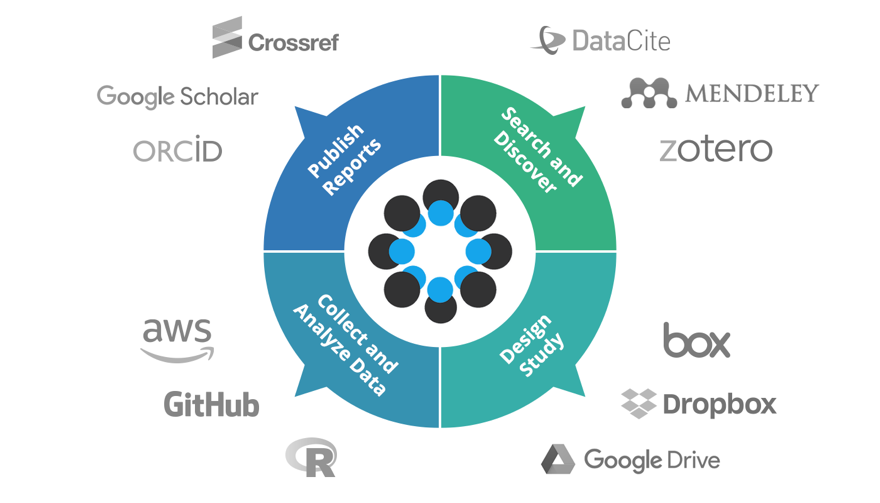
\includegraphics[width=0.5\linewidth]{images/osfframework}
		\caption[Open Science Framework]{Open Science Framework}
		\label{fig:osfframework}
	\end{center}
\end{wrapfigure}
For selecting the suitable instruments for the research, the Open Science Framework\footnote{\url{https://www.cos.io/products/osf}} is used. The Open Science Framework consists out of 4 stages in a research project. Those stages are: ''Search and Discover, Design Study, Collect and Analyse, and Publish Reports.'' The Open Science Framework proposes specific infrastructure and tools per stage. The transparency in the used infrastructure and tools increases the quality of the research. It increases the replication factor, findability, accessibility, interoperability, and reusability.
\subsection{Thesis creation}
\label{sub:tbresearchcreation}
I used my corporate laptop (Dell Latitude 7200 2-in-1\footnote{\url{https://www.dell.com/en-us/work/shop/dell-laptops-and-notebooks/latitude-7200-2-in-1-laptop/spd/latitude-12-7200-2-in-1-laptop}}) with Windows 10 Professional installed for creating the thesis. The thesis is created with the markup language \LaTeX\footnote{\url{https://www.latex-project.org/}}. The used typesetting environment is TexLive\footnote{\url{https://www.tug.org/texlive/}} with the document type of ''Report'' from KOMA-Script\footnote{\url{https://ctan.org/pkg/koma-script}}. TexStudio\footnote{\url{https://www.texstudio.org/}} is the used \LaTeX\ Editor. It supports syntax-highlighting, has an integrated viewer, reference checking and numerous wizards. For the creation and administration of references Bib\LaTeX\footnote{\url{https://ctan.org/pkg/biblatex/}} is used with the reference manager JabRef\footnote{\url{https://www.jabref.org/}} with the citation style of APA 7th Edition\footnote{\url{https://apastyle.apa.org/}} and with web browser integration. The files are stored on a personal Dropbox\footnote{\url{https://www.dropbox.com/}} that is used by GitHub Desktop\footnote{\url{https://desktop.github.com/}} to synchronise with a public GitHub repository\footnote{\url{https://github.com/JRBliekendaal/master-thesis}}. GitHub\footnote{\url{https://github.com/}} is used for source control but also for reviewing and discussing the topics with the (Co-)Promotor and the planning of the master thesis project. The thesis source files are copied to an Amazon S3 Blob\footnote{\url{https://aws.amazon.com/s3/}} for backup. The backup rotation is seven versions. Cloudberry Explorer Freeware for Amazon S3\footnote{\url{https://www.msp360.com/explorer/windows/amazon-s3.aspx}} is used for backup. Grammarly\footnote{\url{https://www.grammarly.com}}, with the paid subscription service, checks the thesis for spelling, grammar,  style, and plagiarism. The used goals for Grammarly are audience=knowledgeable, formality=formal, and domain=academic. Microsoft Visio Professional\footnote{\url{https://www.microsoft.com/en-ww/microsoft-365/visio/}} is used to create figures. The GitHub repository contains all the sources.
\subsection{Research administration}
\label{sub:tbresearchadministration}
The research administration, which includes documentation containing privacy-sensitive information, like the name and contact information of the Delphi Group participants, is stored on a non-public GitHub Repository\footnote{\url{https://github.com/JRBliekendaal/master-thesis-administration}}. The private GitHub Repository is also for staging thesis parts that still need to be anonymised. For taking notes Leuchtturm1917\footnote{\url{https://www.leuchtturm1917.us/notebook-classic.html}} Notebooks are used with mechanical pencils of Faber-Castell\footnote{\url{https://www.fabercastell.com/products/tk-fine-vario-l-mechanical-pencil-10mm-135900}} and pens from Sakura\footnote{\url{https://www.sakuraofamerica.com/product/pigma-micron/}} with long-lasting ink.
\subsection{Research execution}
\label{sub:tbresearchexecution}
For the execution of the research, Microsoft Excel\footnote{\url{https://www.microsoft.com/en-us/microsoft-365/excel}} is used for the administration of the literature research. For the administration of the literature research, the following headers are used: ID (for a unique ID per item), search terms used, scope, title, subtitle, author(s), year, type, Bib\LaTeX\ citation key, title relevance, abstract relevance, content relevance, found at, doi/isbn, url, date found, duplicate, date used, use for, and notes. Researchgate\footnote{\url{https://www.researchgate.net/}}, Web of Science\footnote{\url{https://app.webofknowledge.com/}}, and Google Scholar\footnote{\url{https://scholar.google.com/}} are the main sources for searching for literature. PaperPanda\footnote{\url{https://paperpanda.app/}} is used for hard to find literature. The literature administration is, together with the publicly available literature, stored in the repository of the master thesis. For non-public available literature, the administration contains the location where the literature is retrievable. All the literature is added to a bib\LaTeX\ file for future reference. For traceability the entries in the bib\LaTeX\ file contain the Unique ID in the notes field. JabRef is used to sort the references by using subgroups to support the workflow. The subgroups used are: ''evaluate, rejected, and used.'' Only the literature in the subgroup used are transferred to the bibliography file of the thesis. This prevents cluttering. For working as paperless as possible all the literature, where possible, is in pdf or in ebook format. For reading Acrobat Reader DC\footnote{\url{https://get.adobe.com/reader/}} is used for reading the PDF, and an Amazon Kindle Oasis\footnote{\url{https://www.amazon.com/dp/B07L5GJD99}} for eBooks. With the Amazon Kindle the highlight feature is used. This is not stored on GitHub since the highlights are under copyright of the author(s).\par
For the execution of the Delphi Method, Meetingwizard\footnote{\url{https://www.meetingwizard.nl/}} is used for questionnaires and the analysis of the questionnaires. The license for using Meeting Wizard is supplied by the Antwerp Management School.

\subsection{Summary of used infrastructure and tooling}

\begin{table}[!h]
	\begin{center}
		\begin{tabular}{@{}cccc@{}}
			\toprule
			Search \& Discover & Design Study & Collect \& Analyse Data & Publish Reports\\ \midrule
			Web of Science & 1    & JabRef   & \LaTeX \\%
			ResearchGate   &      &           & TeXstudio \\%
			Google Scholar & 2    & PaperPanda  & ORCID \\%
			Z	 & 0    & bib\LaTeX   & ResearchGate \\%
			Z	 &	x	& Meetingwizard	  & Zenodo \\%
			Z	 &	x	& Microsoft Excel  & Grammarly \\%
			Y    & 2    & GitHub  & Microsoft Visio \\%
			Y	 & 2	& Cloud Berry Explorer for S3 & \\%
			\bottomrule
		\end{tabular}
		\caption{Used infrastructure \& tooling}
		\label{tab:usedinfrastructuretooling}
	\end{center}
\end{table}

\begin{remark}
	This section needs a tabel to summarise the used tools in relation to the OSF framework.
\end{remark}	%	Add the methodology
	%\chapter{Discussion}
\label{ch:discussion}


\section{Discussion on research}
\label{sec:discussiononresearch}


\subsection{Public Sector}
\label{sub:discussionpublicsector}
Is the public sector in The Netherlands the same as in the rest of the world? This needs further research and needs to be confirmed so that the outcome of this research is universally applicable.

\section{Discussion on research quality}
\label{sec:discusssionresearchquality}
\subsection{Size of Delphi Group}
\label{sub:discussionsizeofdelphi}
Is the size of the delphi group large enough to determine....	%	Add the discussion



	\chapter{Chapter Template}
\label{ch:introduction}
\lipsum[1]

\section{section title}
\label{sec:introtitle}
\lipsum[1]
\subsection{subsection title}
\label{subsec:introtitle}
\lipsum[1]
\subsubsection{subsubsection title}
\label{subsubsec:introtitle}
\lipsum[1]
\paragraph{paragraph title}
\label{par:introtitle}
\lipsum[1]
\section{Building Blocks}
\subsection{table}
\begin{table}[!h]
	\begin{center}
		\begin{tabular}{@{}ccccc@{}}
			\toprule
			What & When & Who & Why & How \\ \midrule
			X    & 1    & 1   & 2   & 3   \\
			Y    & 2    & 45  & 7   & 9   \\
			Z    & 0    & 0   & 1   & 7   \\ \bottomrule
		\end{tabular}
		\caption{Introduction Table}
		\label{tab:introduction}
	\end{center}
\end{table}
\subsection{Picture}
\begin{figure}[!h]
	\centering
	
\includegraphics[width=6cm]{images/placeholder-image}
	\caption[Placeholder]{Placeholder}
	\label{fig:placeholder-image}
\end{figure}
\subsection{Glossary}

\gls{antifragile} is not that \gls{fragile}\\
\Gls{antifragile} is not that \Gls{fragile}\\
\gls{fragile} is not that \gls{antifragile}\\
\Gls{fragile} is not that \Gls{antifragile}\\

\subsection{Abbreviation}

\acrfull{vuca}\\
\acrlong{vuca}\\
\acrshort{vuca}\\

\subsection{Citing}
\begin{verbatim*}
	\parencite{Bliek2017}
	\citeyear{Bliek2017}
	\citeauthor{Bliek2017}
\end{verbatim*}
Gives:\\
\parencite{Bliek2017}\\
\citeyear{Bliek2017}\\
\citeauthor{Bliek2017}
	%	Add the Chapter Template

	% Tail of Thesis
	
	\printbibliography				%	Add Bibliography

	\begin{appendices}
		\chapter{Interview Participants}
\label{app:interviewparticipants}

\begin{table}[!h]
	\begin{center}
		\begin{tabular}{@{}ccccc@{}}
			\toprule
			\textbf{Who} & \textbf{Role} & \textbf{From} \\ \midrule
			Christiaan Konstapel & Lead Enterprise Architect & Mileway \\
			Y    & 2    & tbd \\
			Y    & 2    & tbd \\ \bottomrule
		\end{tabular}
		\caption{Interview Participants}
		\label{tab:interviewparticipants}
	\end{center}
\end{table}
		\chapter{Delphi Group Participants}
\label{app:delphigroupparticipants}

\begin{table}[!h]
	\begin{center}
		\begin{tabular}{@{}ccccc@{}}
			\toprule
			\textbf{Who} & \textbf{Role} & \textbf{From} \\ \midrule
			Jan Ploeg & Enterprise Architect & Centric Netherlands B.V. (ISV) \\
			Y    & 2    & Other ISV \\
			Y    & 2    & Municipality \\
			Y    & 2    & VNG-Realisatie \\
			Y    & 2    & Logius \\
			Z    & 0    & Academic \\ \bottomrule
		\end{tabular}
		\caption{Delphi Group Participants}
		\label{tab:delphigroupparticipants}
	\end{center}
\end{table}
		\chapter{Literature Selection}
\label{app:literature_selection}


		\chapter{Research Log}
\label{app:researchlog}

\begin{table}[!h]
	\begin{center}
		\begin{tabularx}{\textwidth}{@{}lX@{}}
			\toprule
			\textbf{Date} & \textbf{What} \\ \midrule%
			24/11/20 & Initial research subject proposal to AMS \\%
			25/11/20 & Initial research subject proposal sent to Hans Mulder \& Yuri Bobbert \\%
			30/11/20 & First meeting with Hans Mulder to explore the subject \\%
			12/02/21 & AMS Master Project Coaching \\%
			10/03/21 & Second meeting with Hans Mulder. Definitive Area of Research selected. The success factors of EA for Business Agility/Resilience/antifragility \\%			
			11/03/21 & Elaborated with COO on antifragility \\%
			14/03/21 & Started research on the concept of antifragility \\%
			03/04/21 & One Pager on the concepts Enterprise Architecture, Public Sector, Independant Software Vendor, and Antifragility \\%			
			04/04/21 & Deskresearch on concepts \\%			
			10/04/21 & Reading Taleb \\%			
			25/05/21 & Third meeting with Hans Mulder \\%	
			20/06/21 & Creating 5 pager \\%
			20/06/21 & Sent 5 pager presentation for review to Hans Mulder \\%
			20/06/21 & Sent 5 pager presentation for review to Dieneke Schouten (COO) and Maarten Hillenaar (CEO) \\%
			20/06/21 & Promotor suggestion Roland Ettema, Martin Op 't Land, Bas van Gils or Hans Mulder \\%
			20/06/21 & Sugestion of Hans Mulder as promotor with Edzo Botjes as co-promotor \\%
			21/06/21 & Requested Maarten Hillenaar as Sponsor, Dieneke Schouten as Second Reader, Jan Ploeg as participant in Delphi, Christiaan Konstapel as interviewee \\%			
			24/06/21 & Presentation of Five Pager at Master Project Coaching AMS \\%
			29/06/21 & Created thesis LaTeX skeleton  \\%			
			06/07/21 & Meeting with Edzo Botjes to get acquainted \\%	
			06/07/21 & Edzo Botjes accepted co-promotorship \\%
			date    & what \\%
			date    & what \\%
			date    & what \\%
			enddate & final version \\ \bottomrule
		\end{tabularx}
		\label{tab:researchlog}
	\end{center}
\end{table}
	\end{appendices}

\end{document}